\chapter{Transición. Cosas} \label{cap:transition_apendice}

\subsection{Autofunciones y Espectros de autovalores}

\textcolor{red}{LAS AUTOFUNCIONES ESTÁN MAL. HAY QUE CAMBIARLAS, REVISAR LAS AUTENTICAS. ADEMAS, HAY UN TEMA DE LA SIMETRÍA, ESTÁN ESPEJEDAS RESPECTO AL EJE Y.}

\begin{figure}[H]
  \centering
  \subfloat[]{
    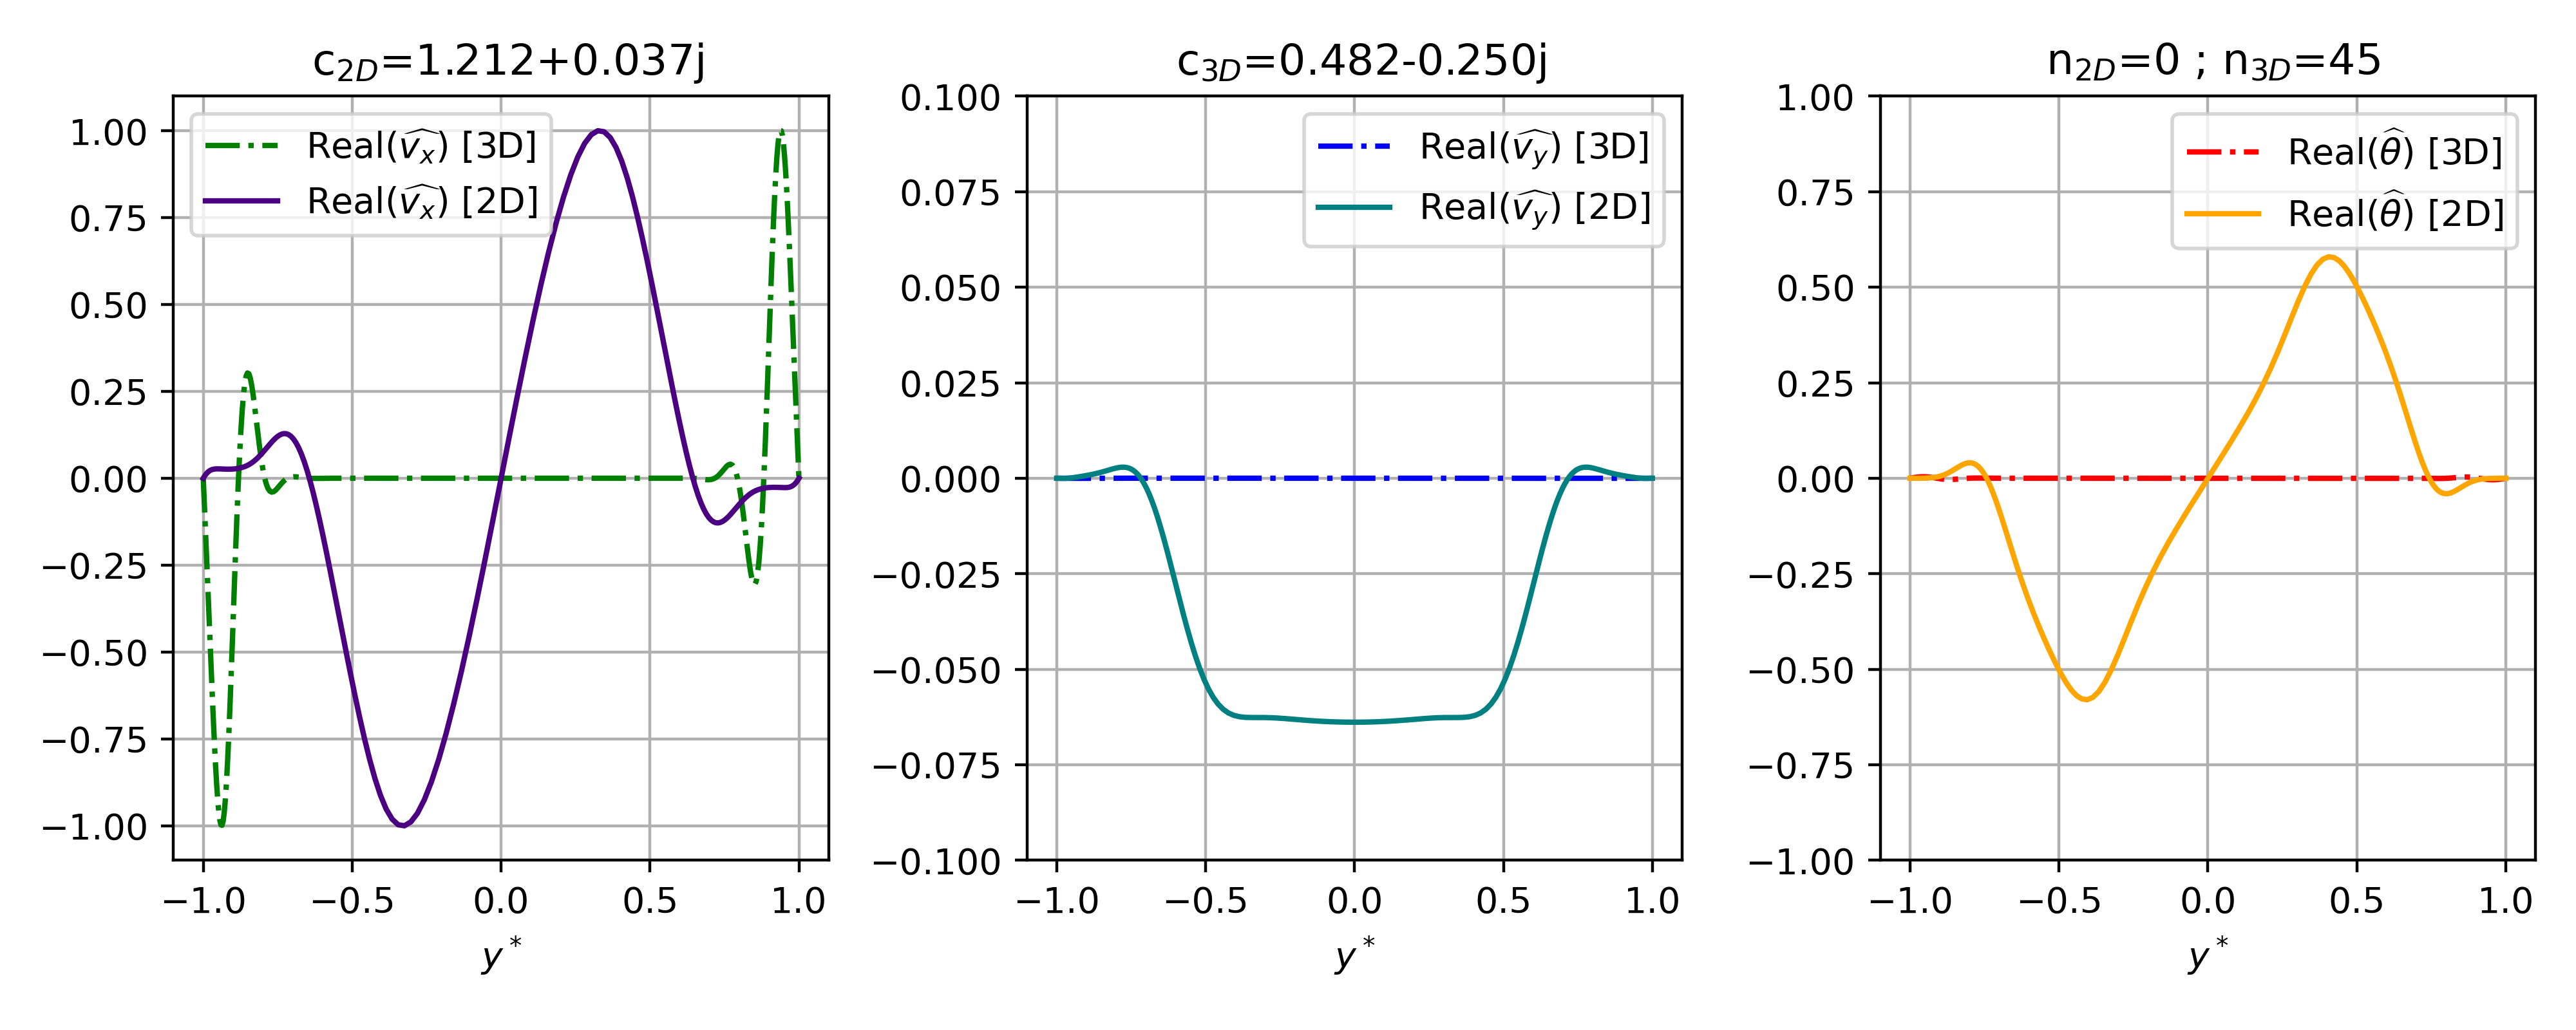
\includegraphics[width=\textwidth]{figures/cap6/Re5000-Pr071-Ri1Em6/Re5000-Pr071-Ri1Em6_eigenfun_A2.png}}
  \caption{}
  \label{fig:eigenfuns1-Re5000-Pr0071}
\end{figure}

\begin{figure}[H]
  \centering    
  \subfloat[]{
    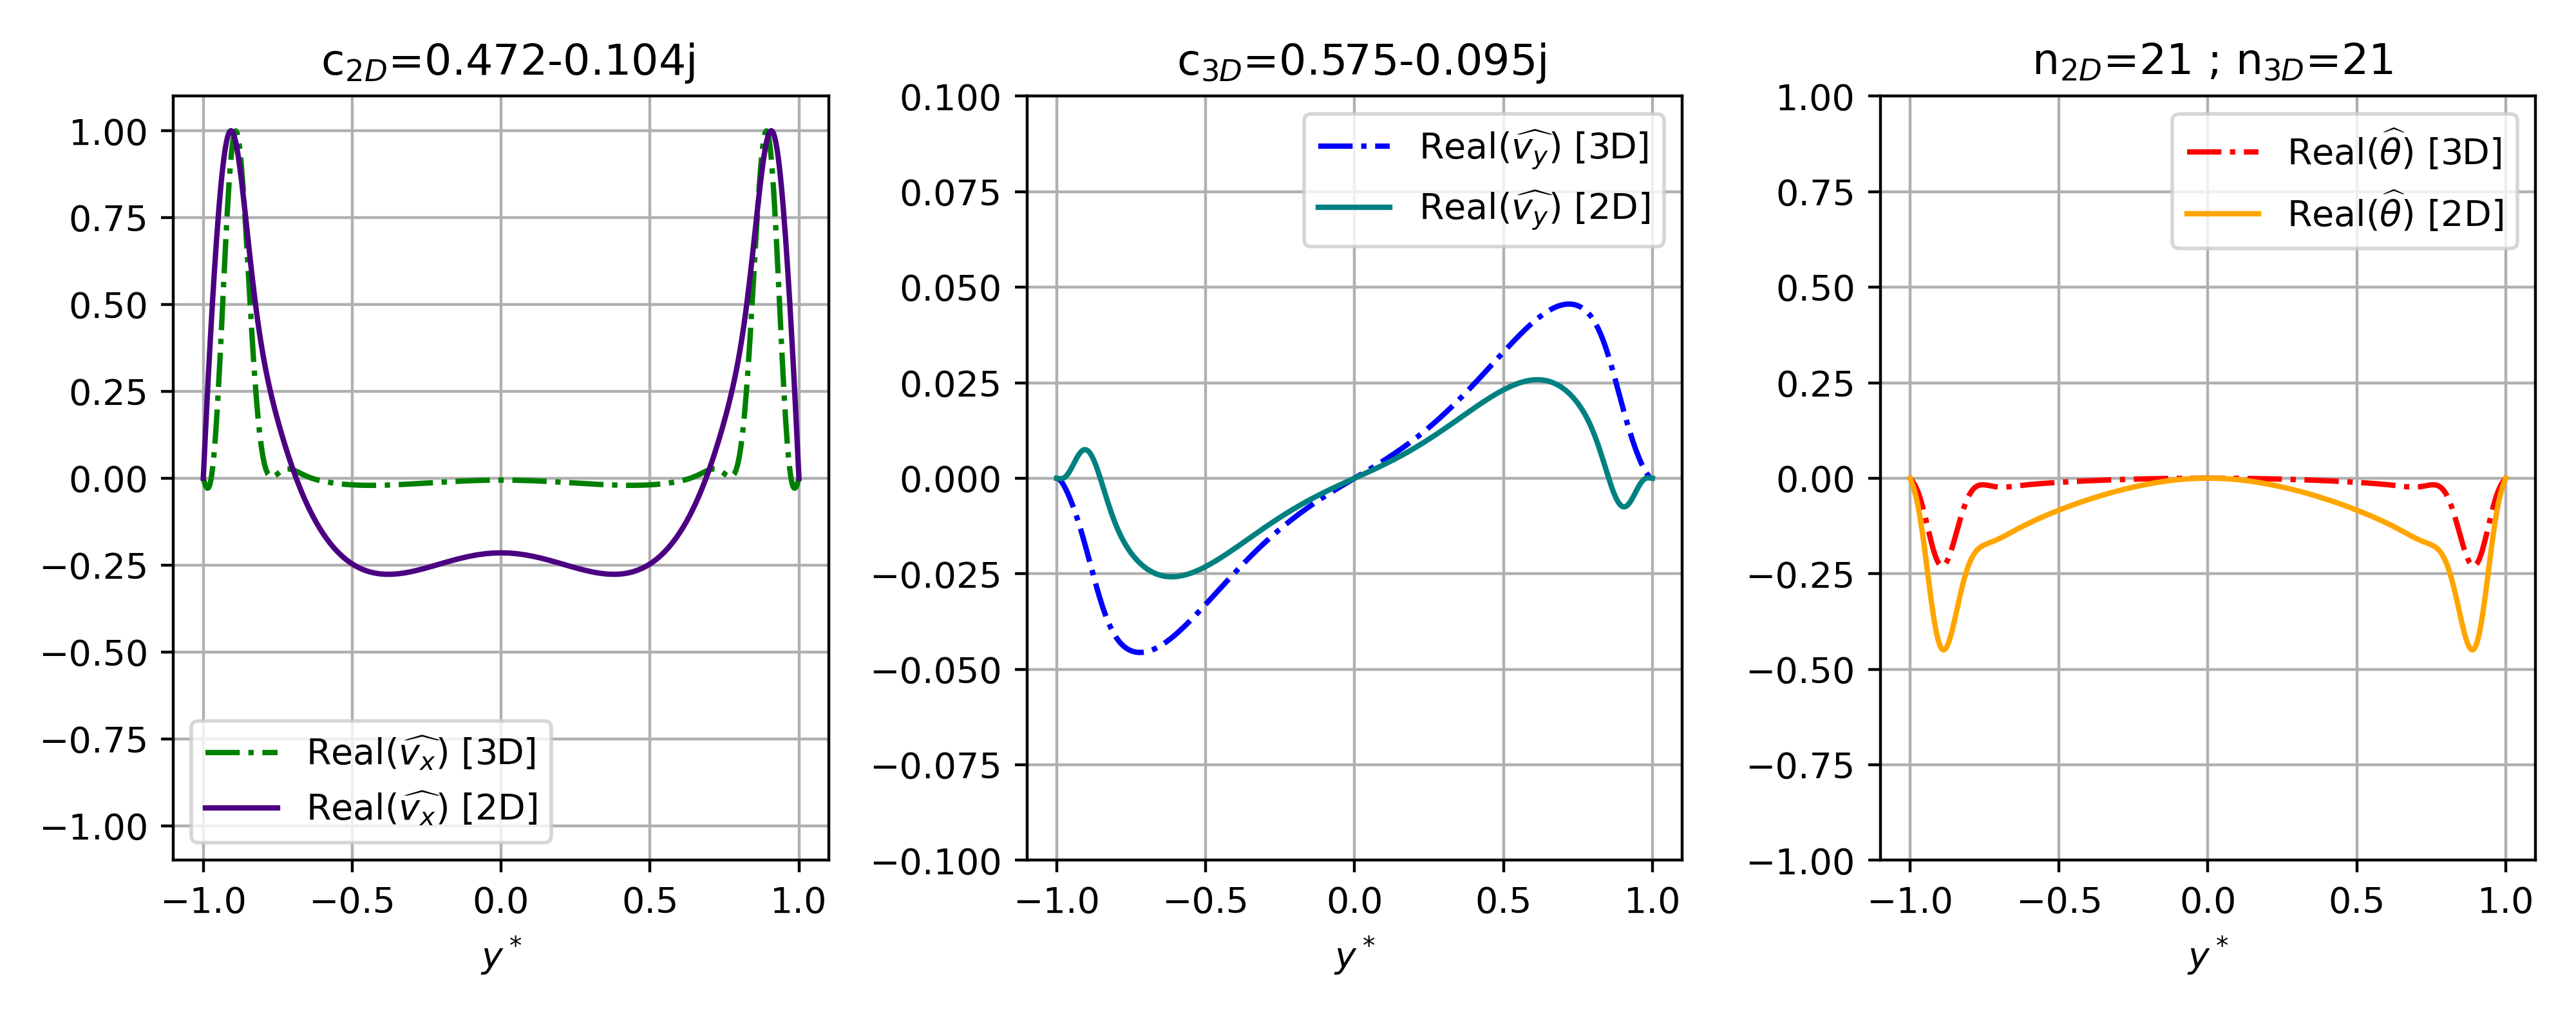
\includegraphics[width=\textwidth]{figures/cap6/Re5000-Pr071-Ri1Em6/Re5000-Pr071-Ri1Em6_eigenfun_A5.png}}
  \caption{}
  \label{fig:eigenfuns2-Re5000-Pr0071}
\end{figure}

\begin{figure}[H]
  \centering  
  \subfloat[]{
    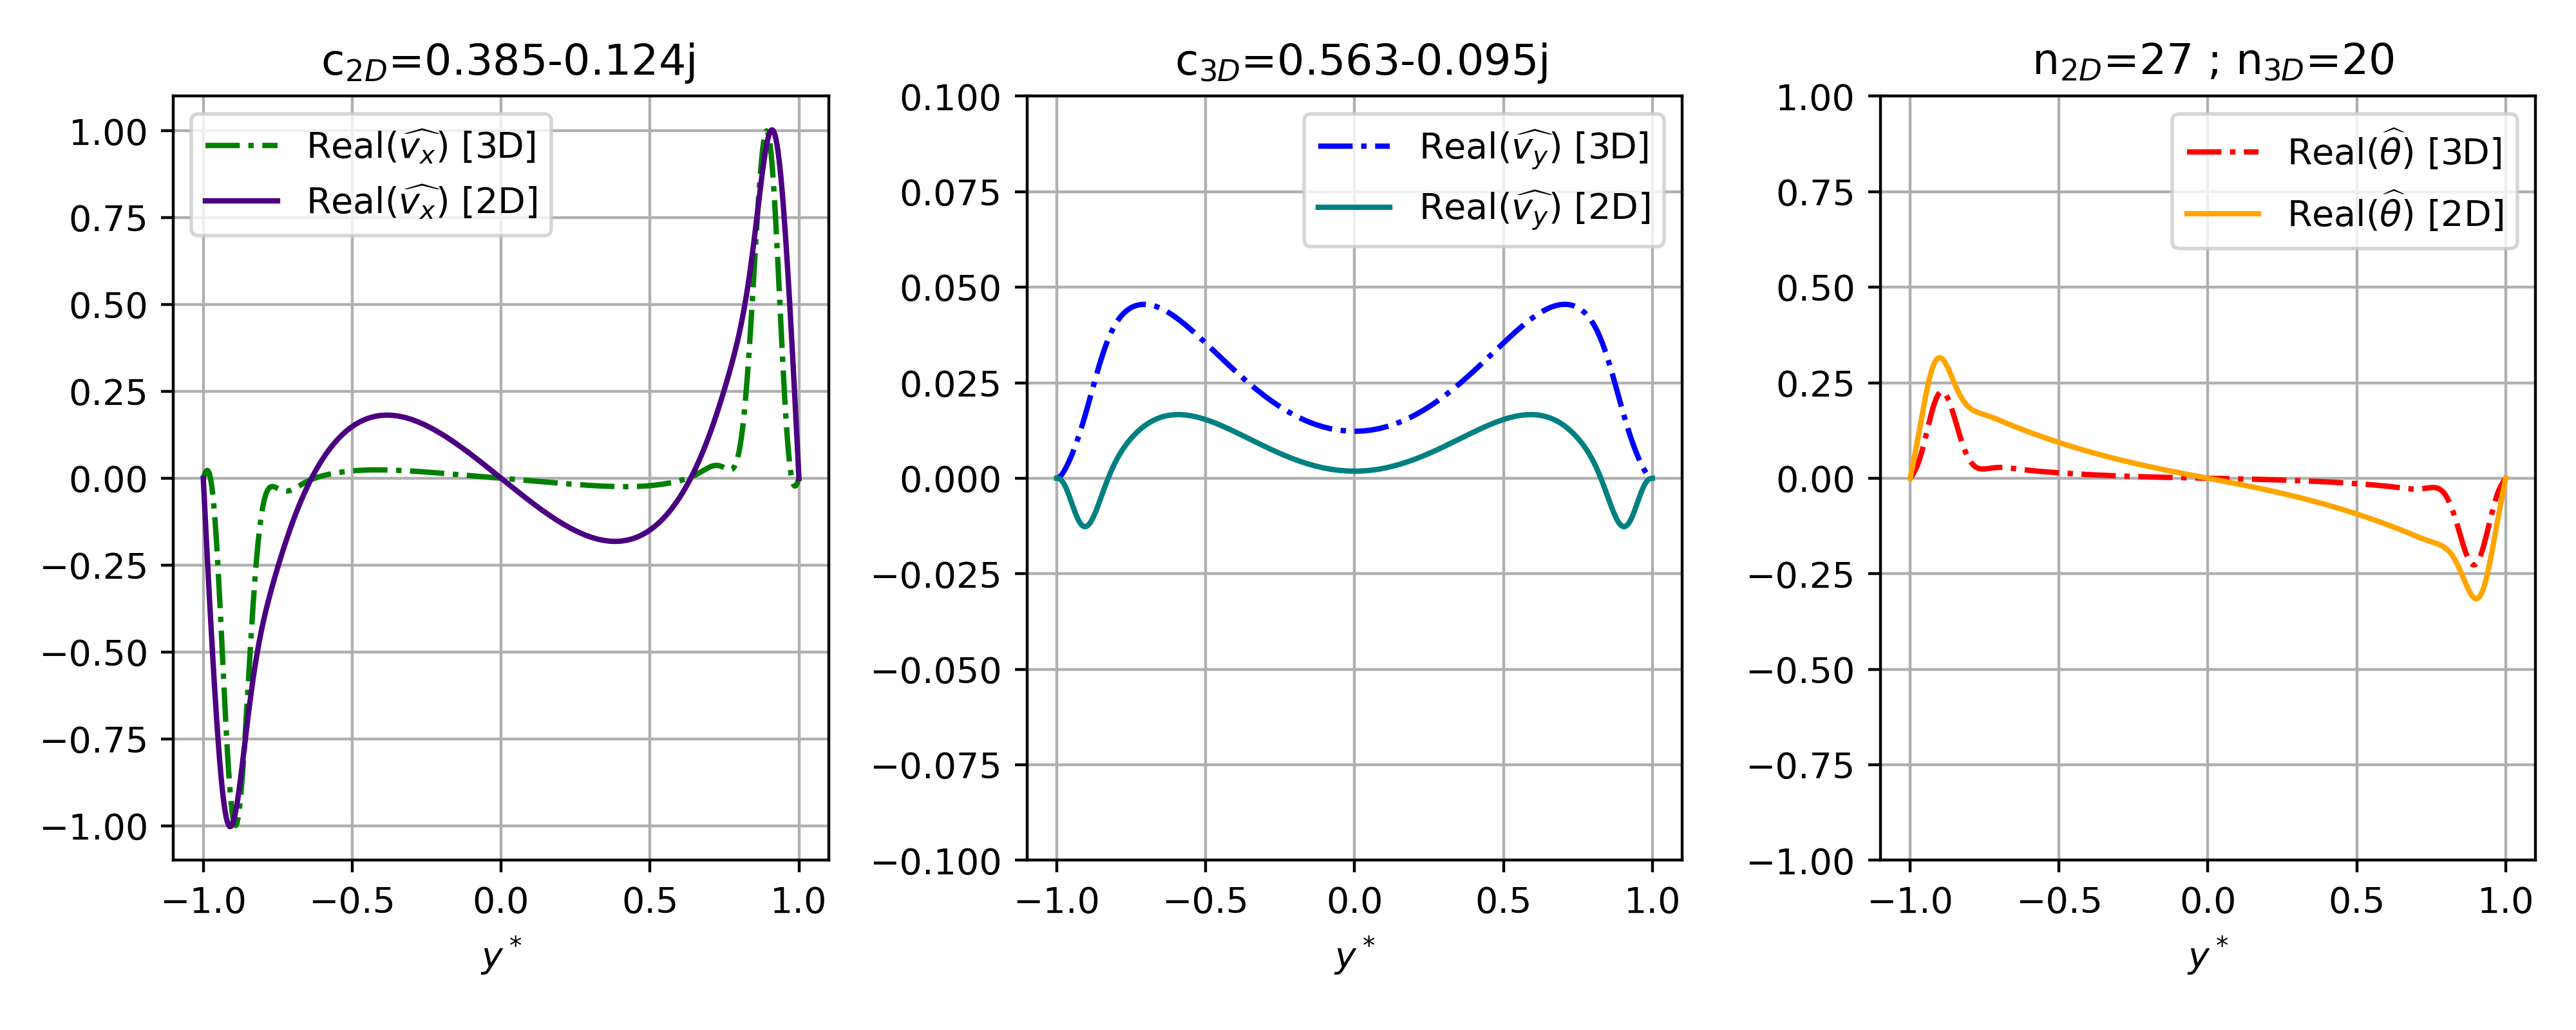
\includegraphics[width=\textwidth]{figures/cap6/Re5000-Pr071-Ri1Em6/Re5000-Pr071-Ri1Em6_eigenfun_A6.png}}
  \caption{}
  \label{fig:eigenfuns3-Re5000-Pr0071}
\end{figure}

\begin{figure}[H]
  \centering  
  \subfloat[]{
    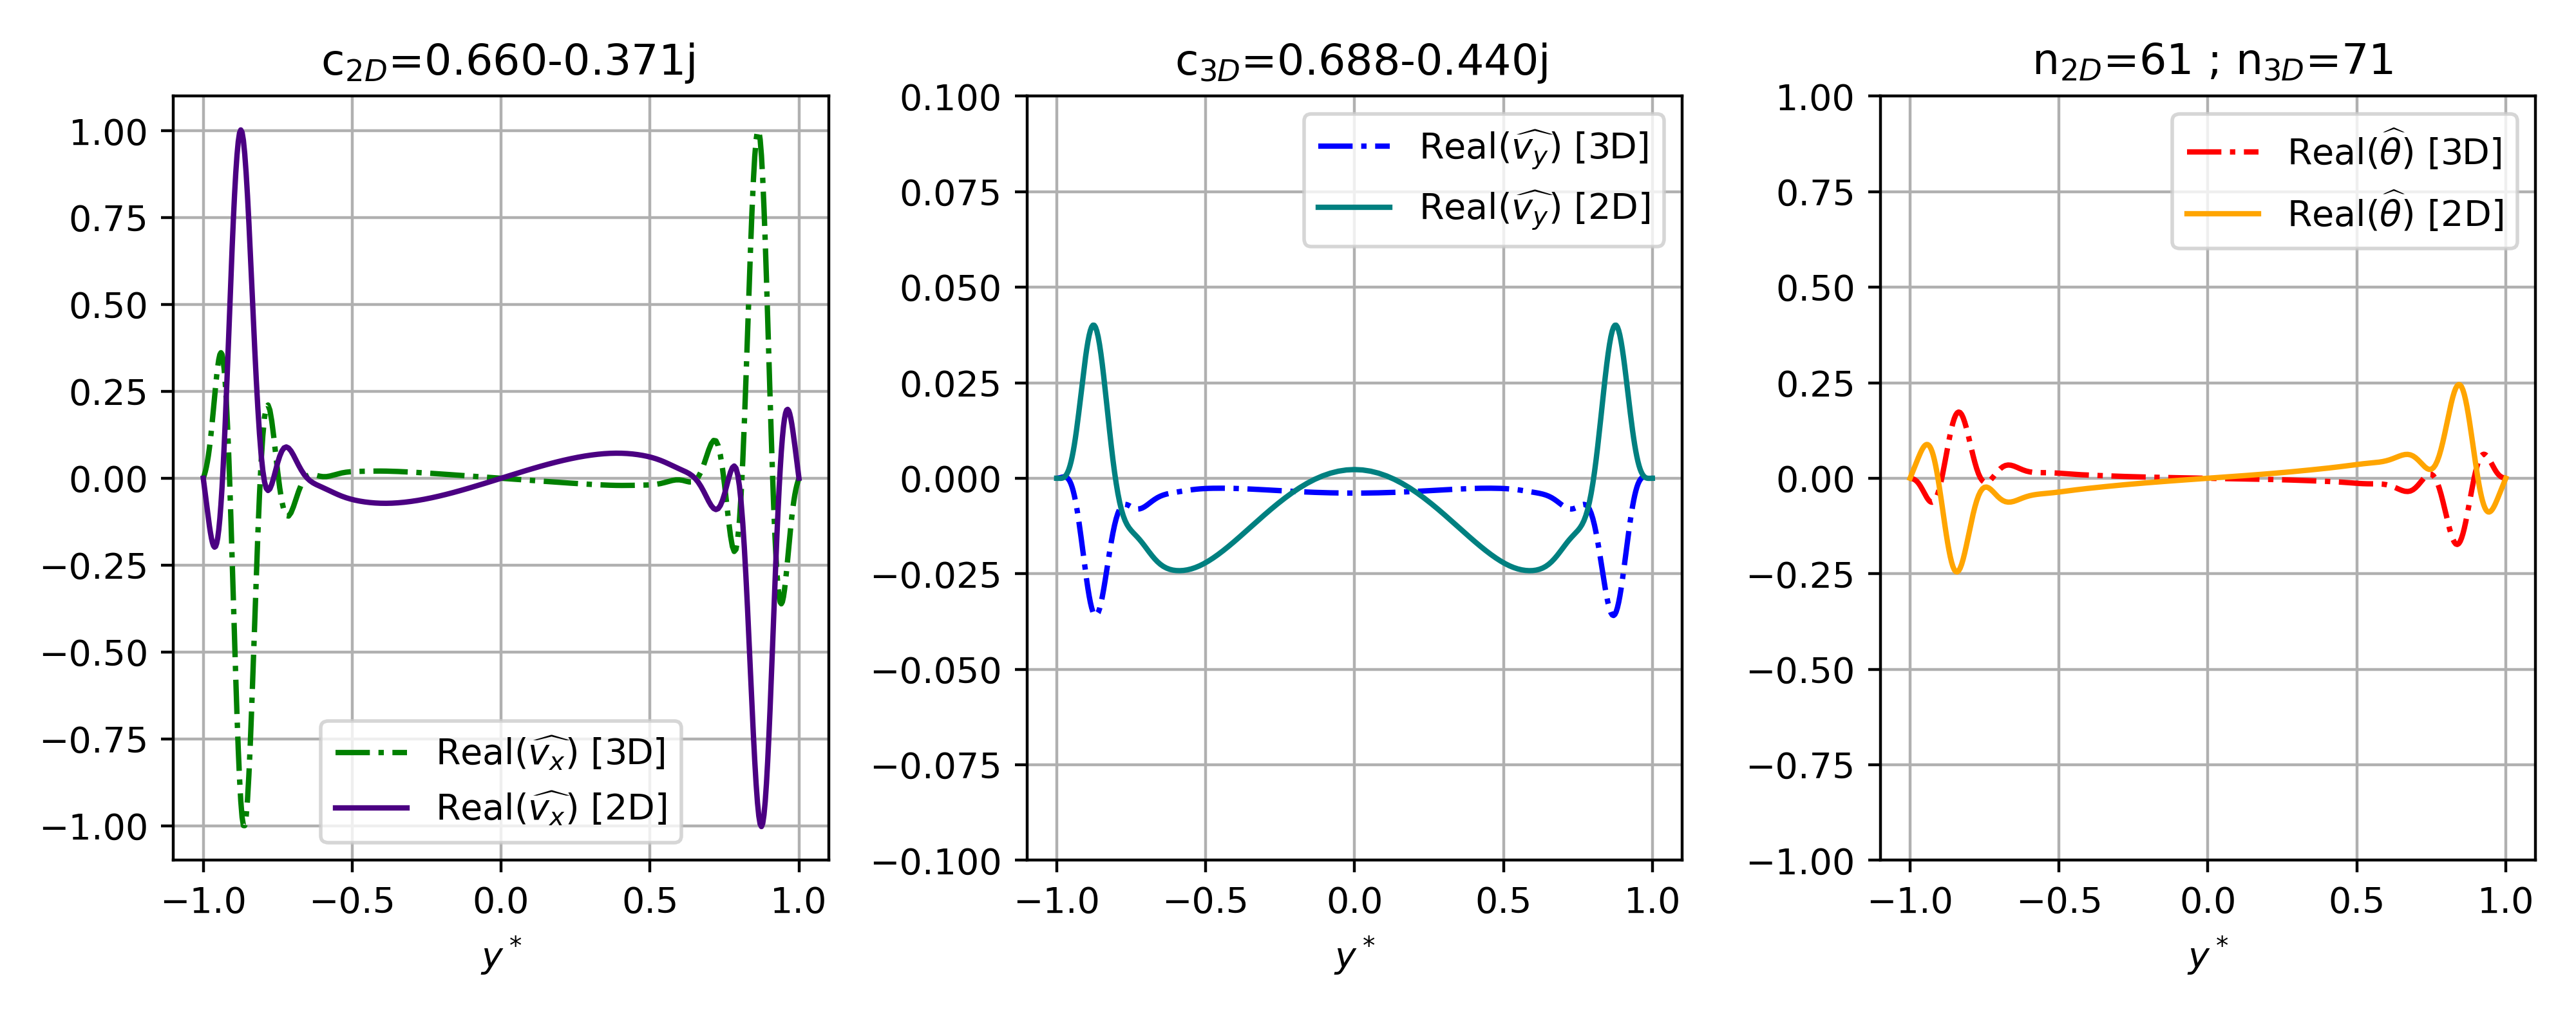
\includegraphics[width=\textwidth]{figures/cap6/Re5000-Pr071-Ri1Em6/Re5000-Pr071-Ri1Em6_eigenfun_A7.png}}

  \caption{}
  \label{fig:eigenfuns4-Re5000-Pr0071}
\end{figure}

\begin{figure}[H]
  \centering
    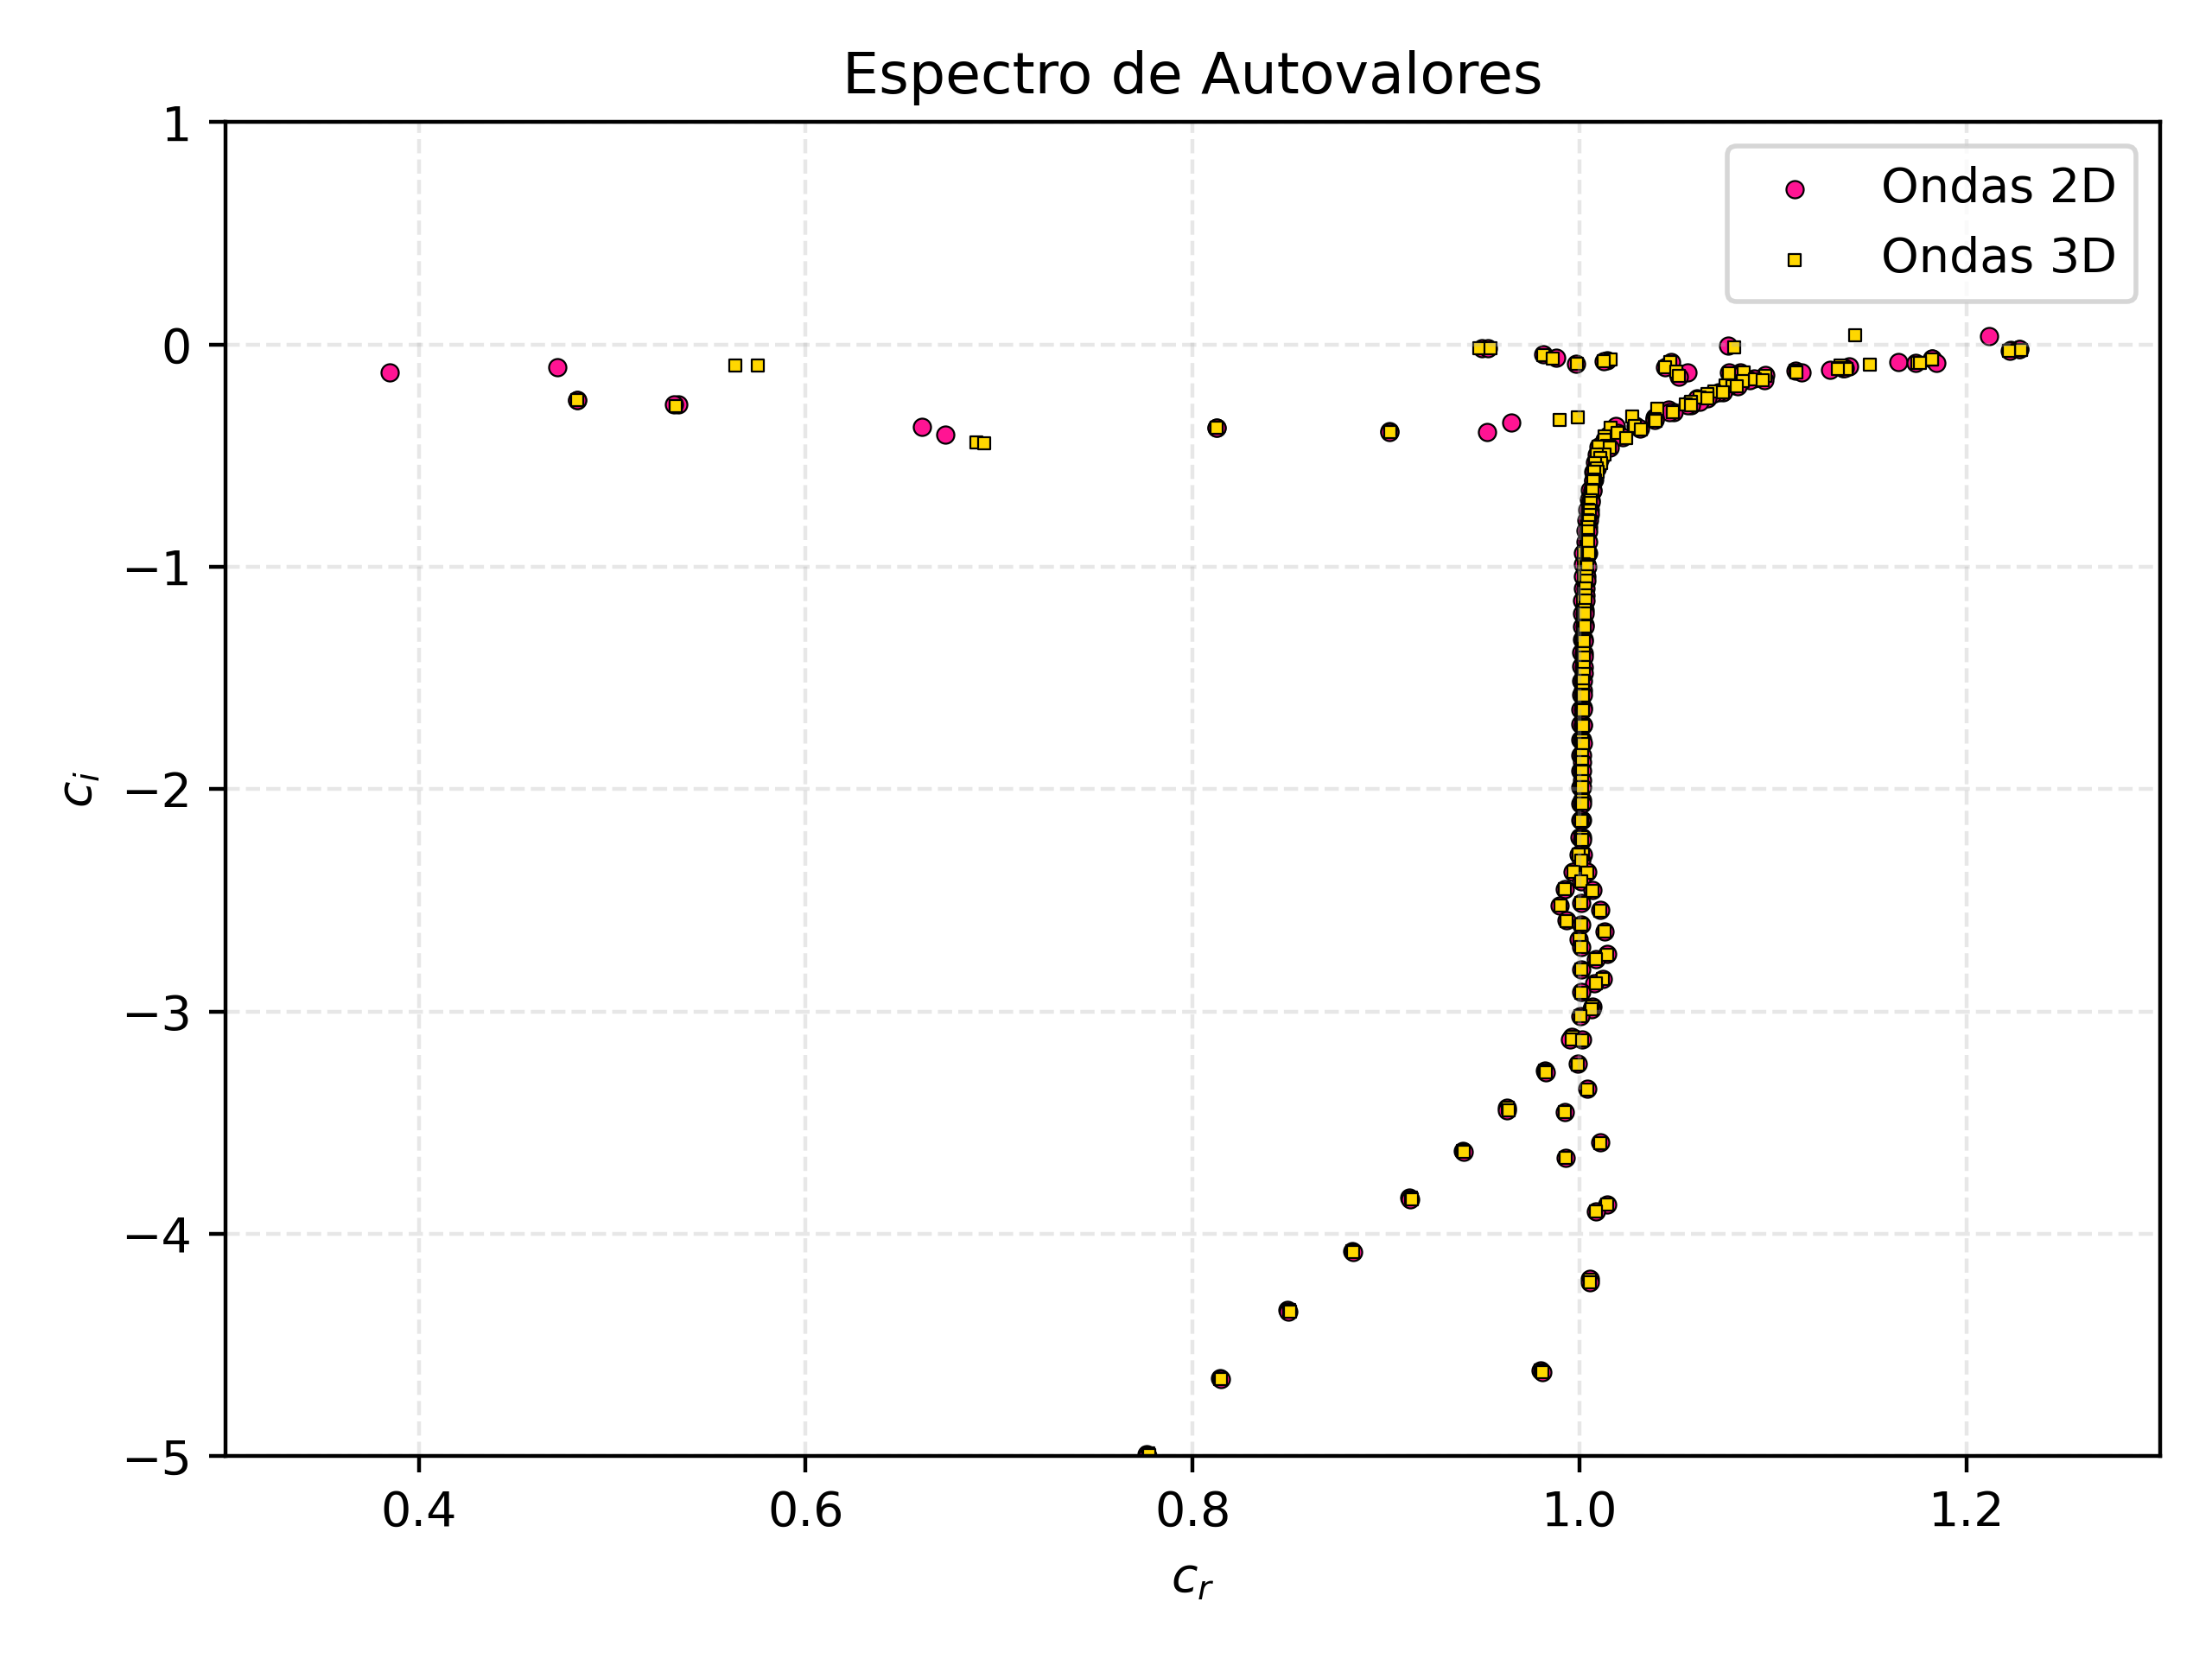
\includegraphics[width=0.6\textwidth]{figures/cap6/Re5000-Pr071-Ri1Em6/Re5000-Pr071-Ri1Em6_eigenvals.png}
  \caption{}
  \label{fig:spectra-Re5000-Pr0071}
\end{figure}


\newpage

\section{Casos $\text{Re}=5000$ ; $\text{Pr}=0.71$ ; $\Pi=10^{-4}$}

\subsection{Autofunciones y Espectros de autovalores}

\begin{figure}[H]
  \centering
  \subfloat[]{
    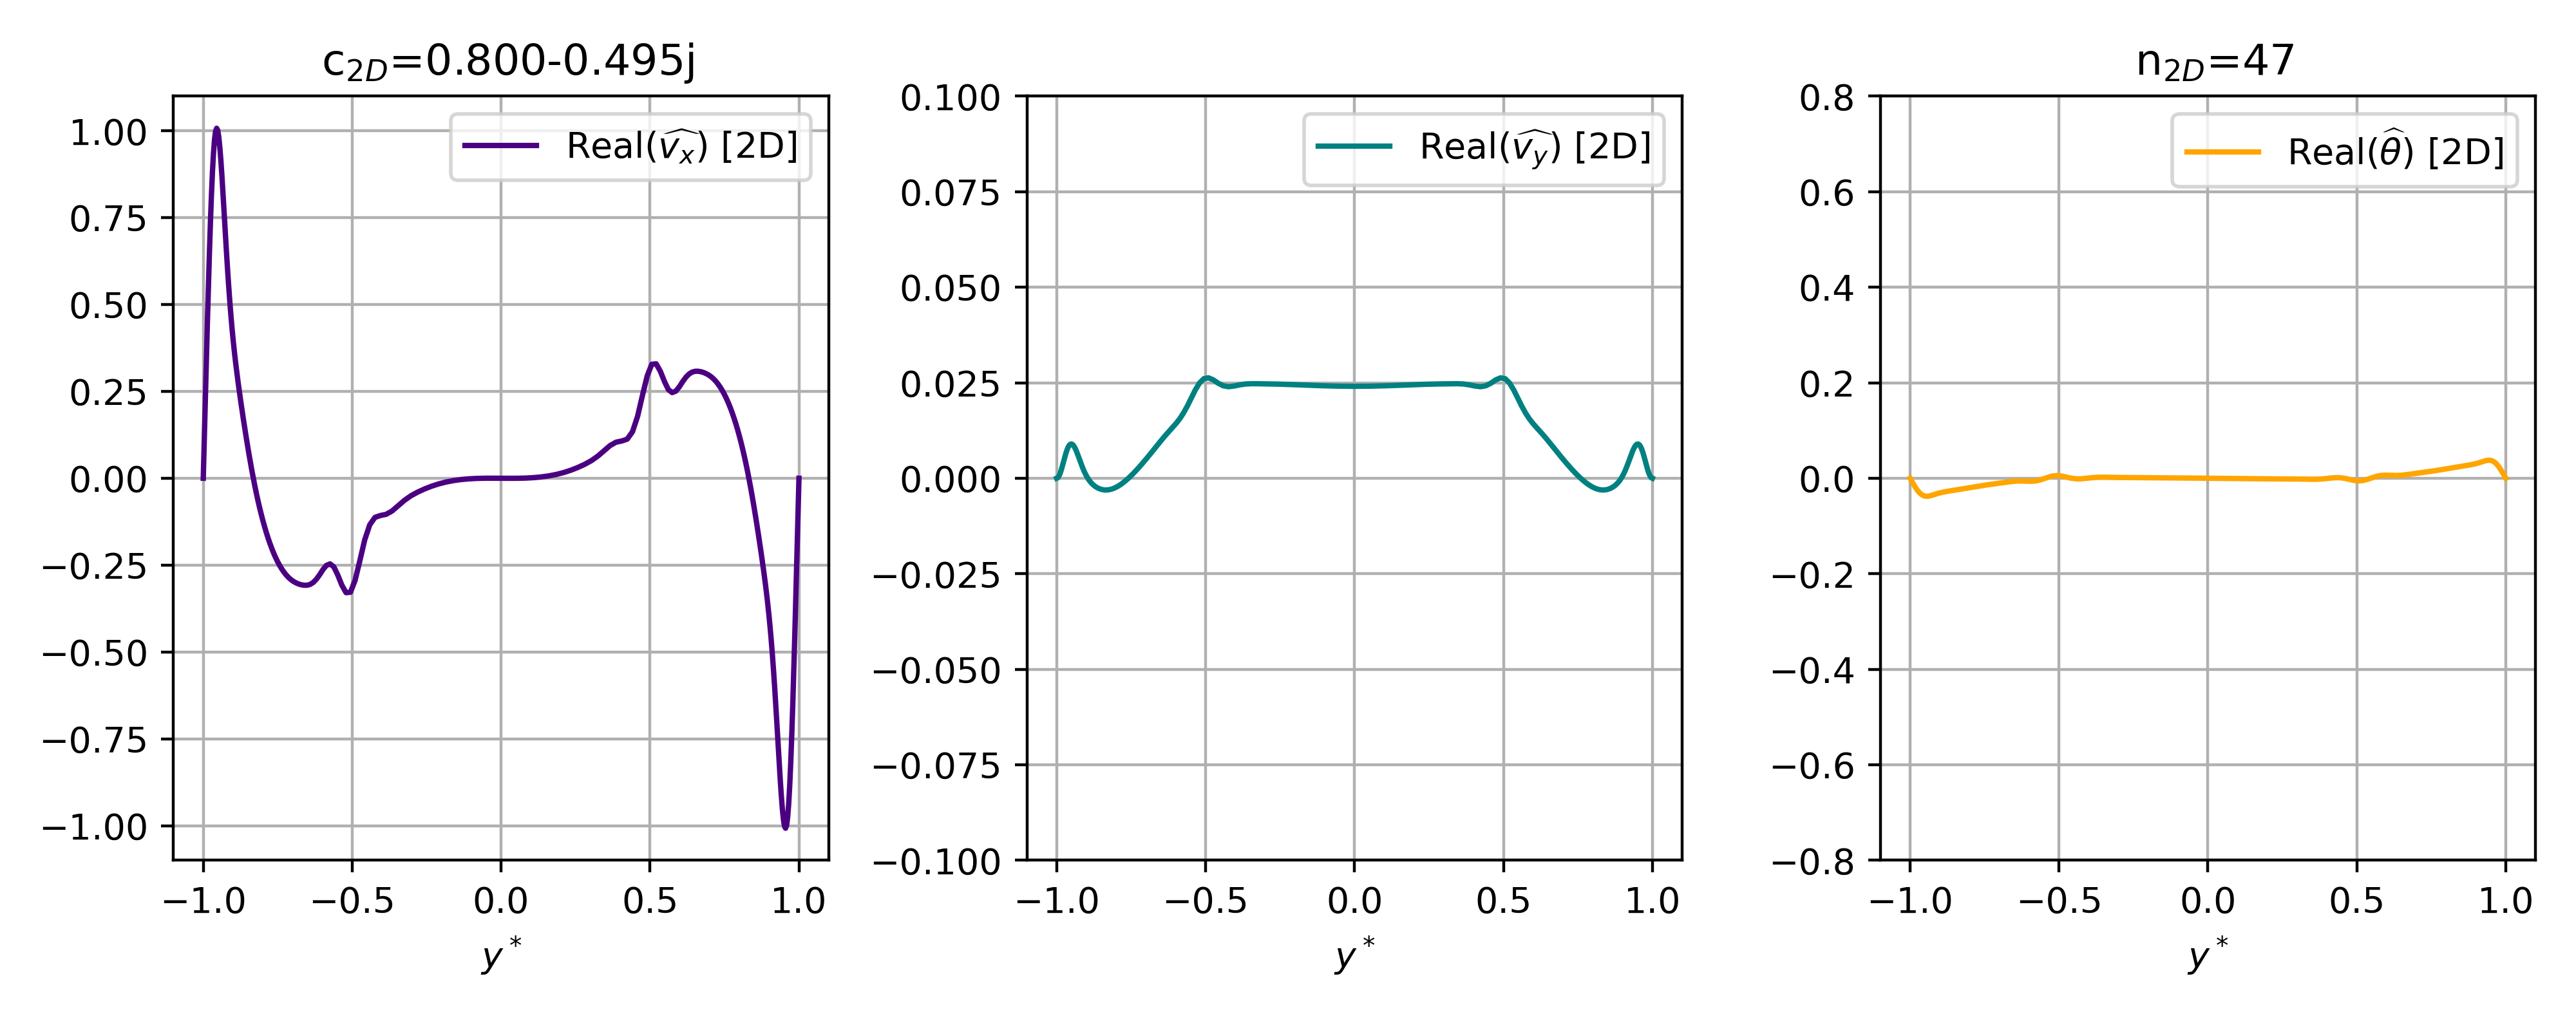
\includegraphics[width=\textwidth]{figures/cap6/Re5000-Pr071-Ri1Em4/Re5000-Pr071-Ri1Em4_eigenfun_A1.png}}
  \caption{}
  \label{fig:eigenfuns1-Re5000-Pr0071}
\end{figure}

\begin{figure}[H]
  \centering    
  \subfloat[]{
    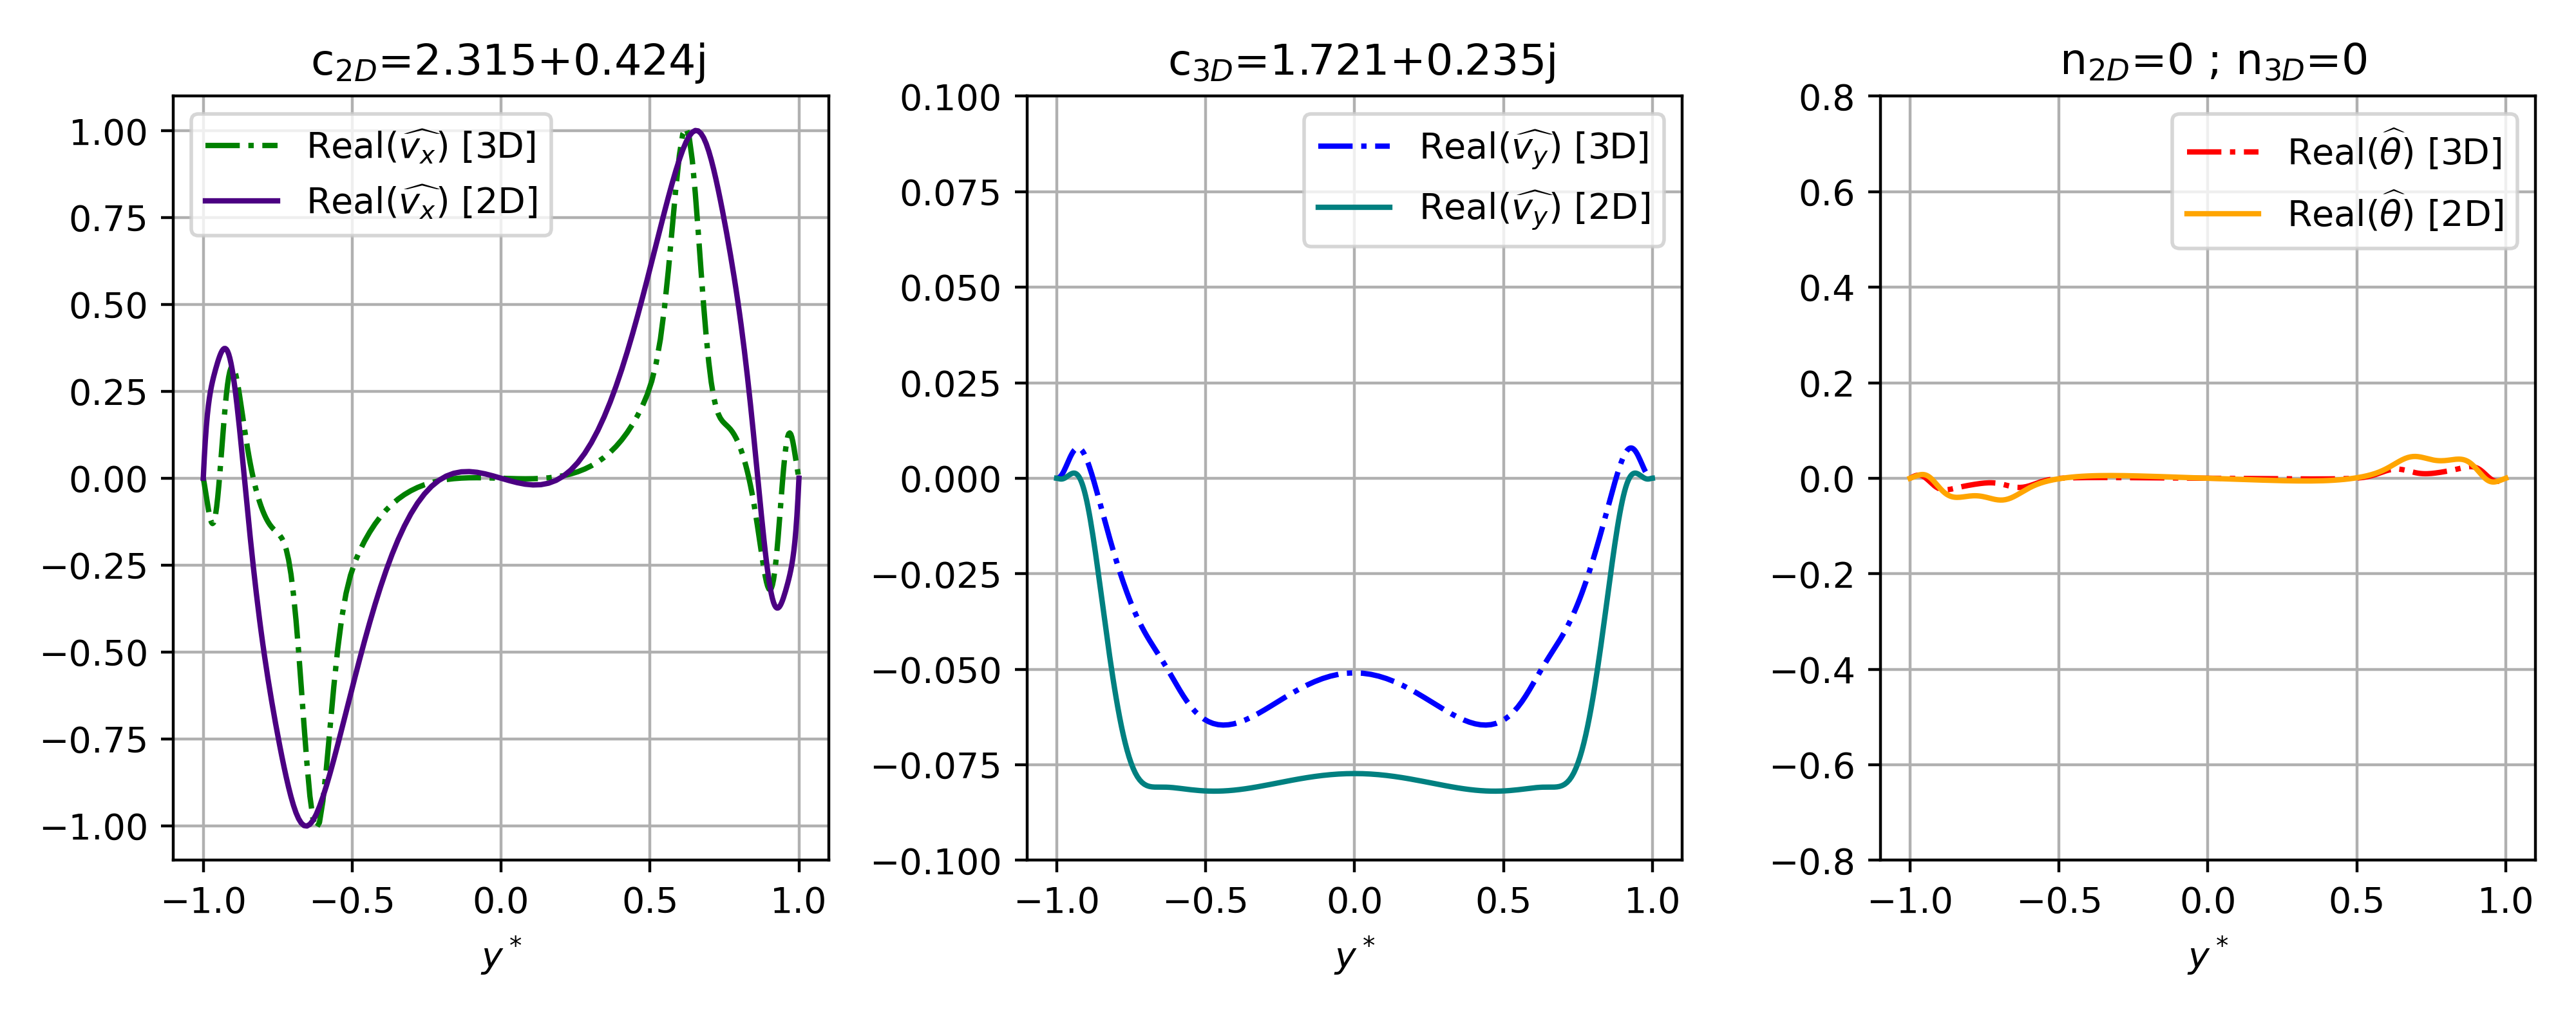
\includegraphics[width=\textwidth]{figures/cap6/Re5000-Pr071-Ri1Em4/Re5000-Pr071-Ri1Em4_eigenfun_A3.png}}
  \caption{}
  \label{fig:eigenfuns2-Re5000-Pr0071}
\end{figure}

\begin{figure}[H]
  \centering  
  \subfloat[]{
    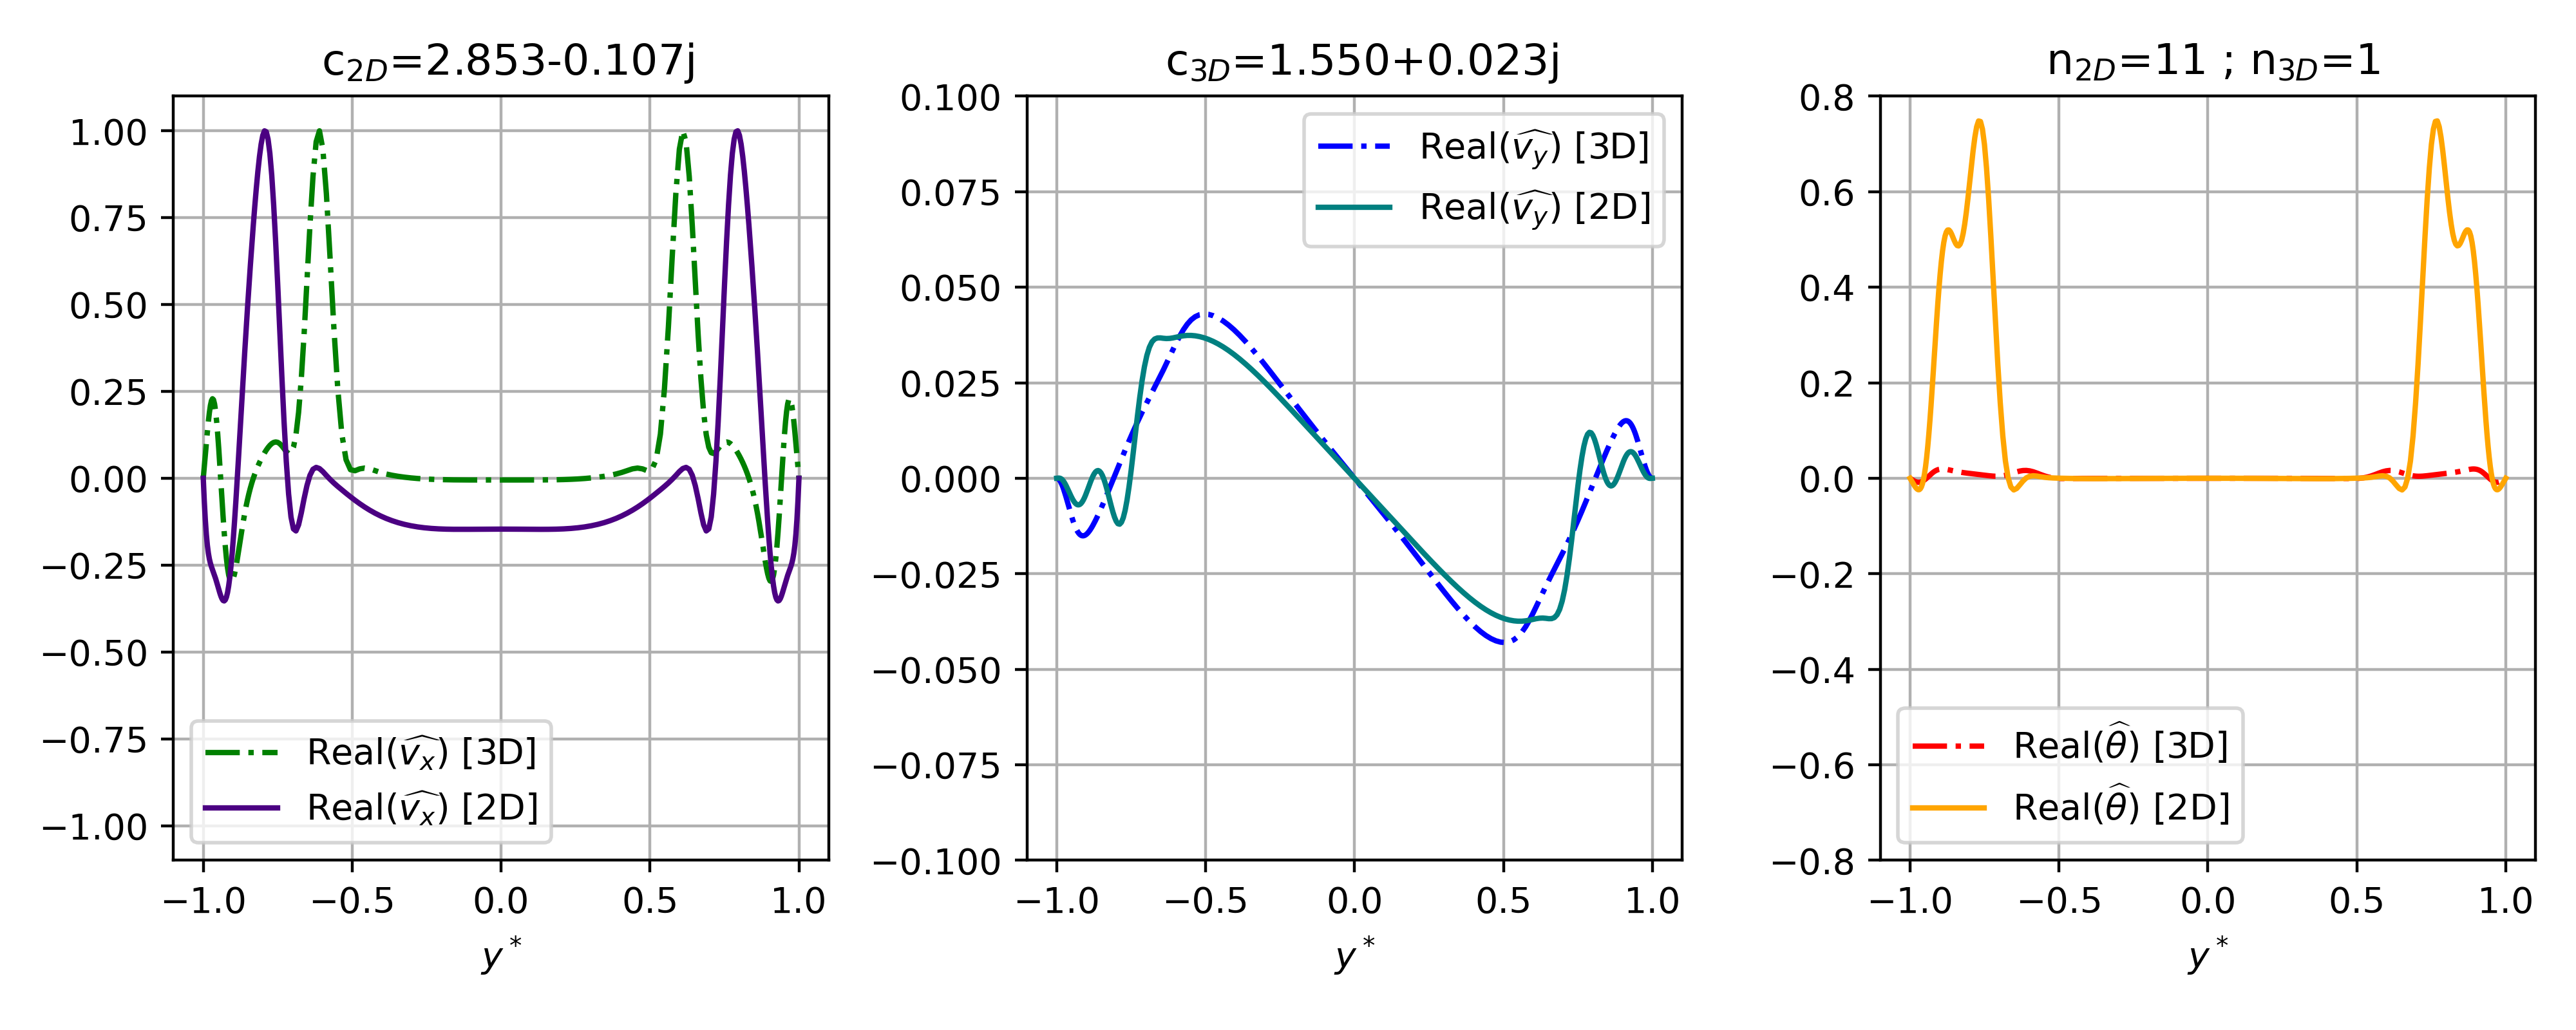
\includegraphics[width=\textwidth]{figures/cap6/Re5000-Pr071-Ri1Em4/Re5000-Pr071-Ri1Em4_eigenfun_A4.png}}
  \caption{}
  \label{fig:eigenfuns3-Re5000-Pr0071}
\end{figure}


\begin{figure}[H]
  \centering
    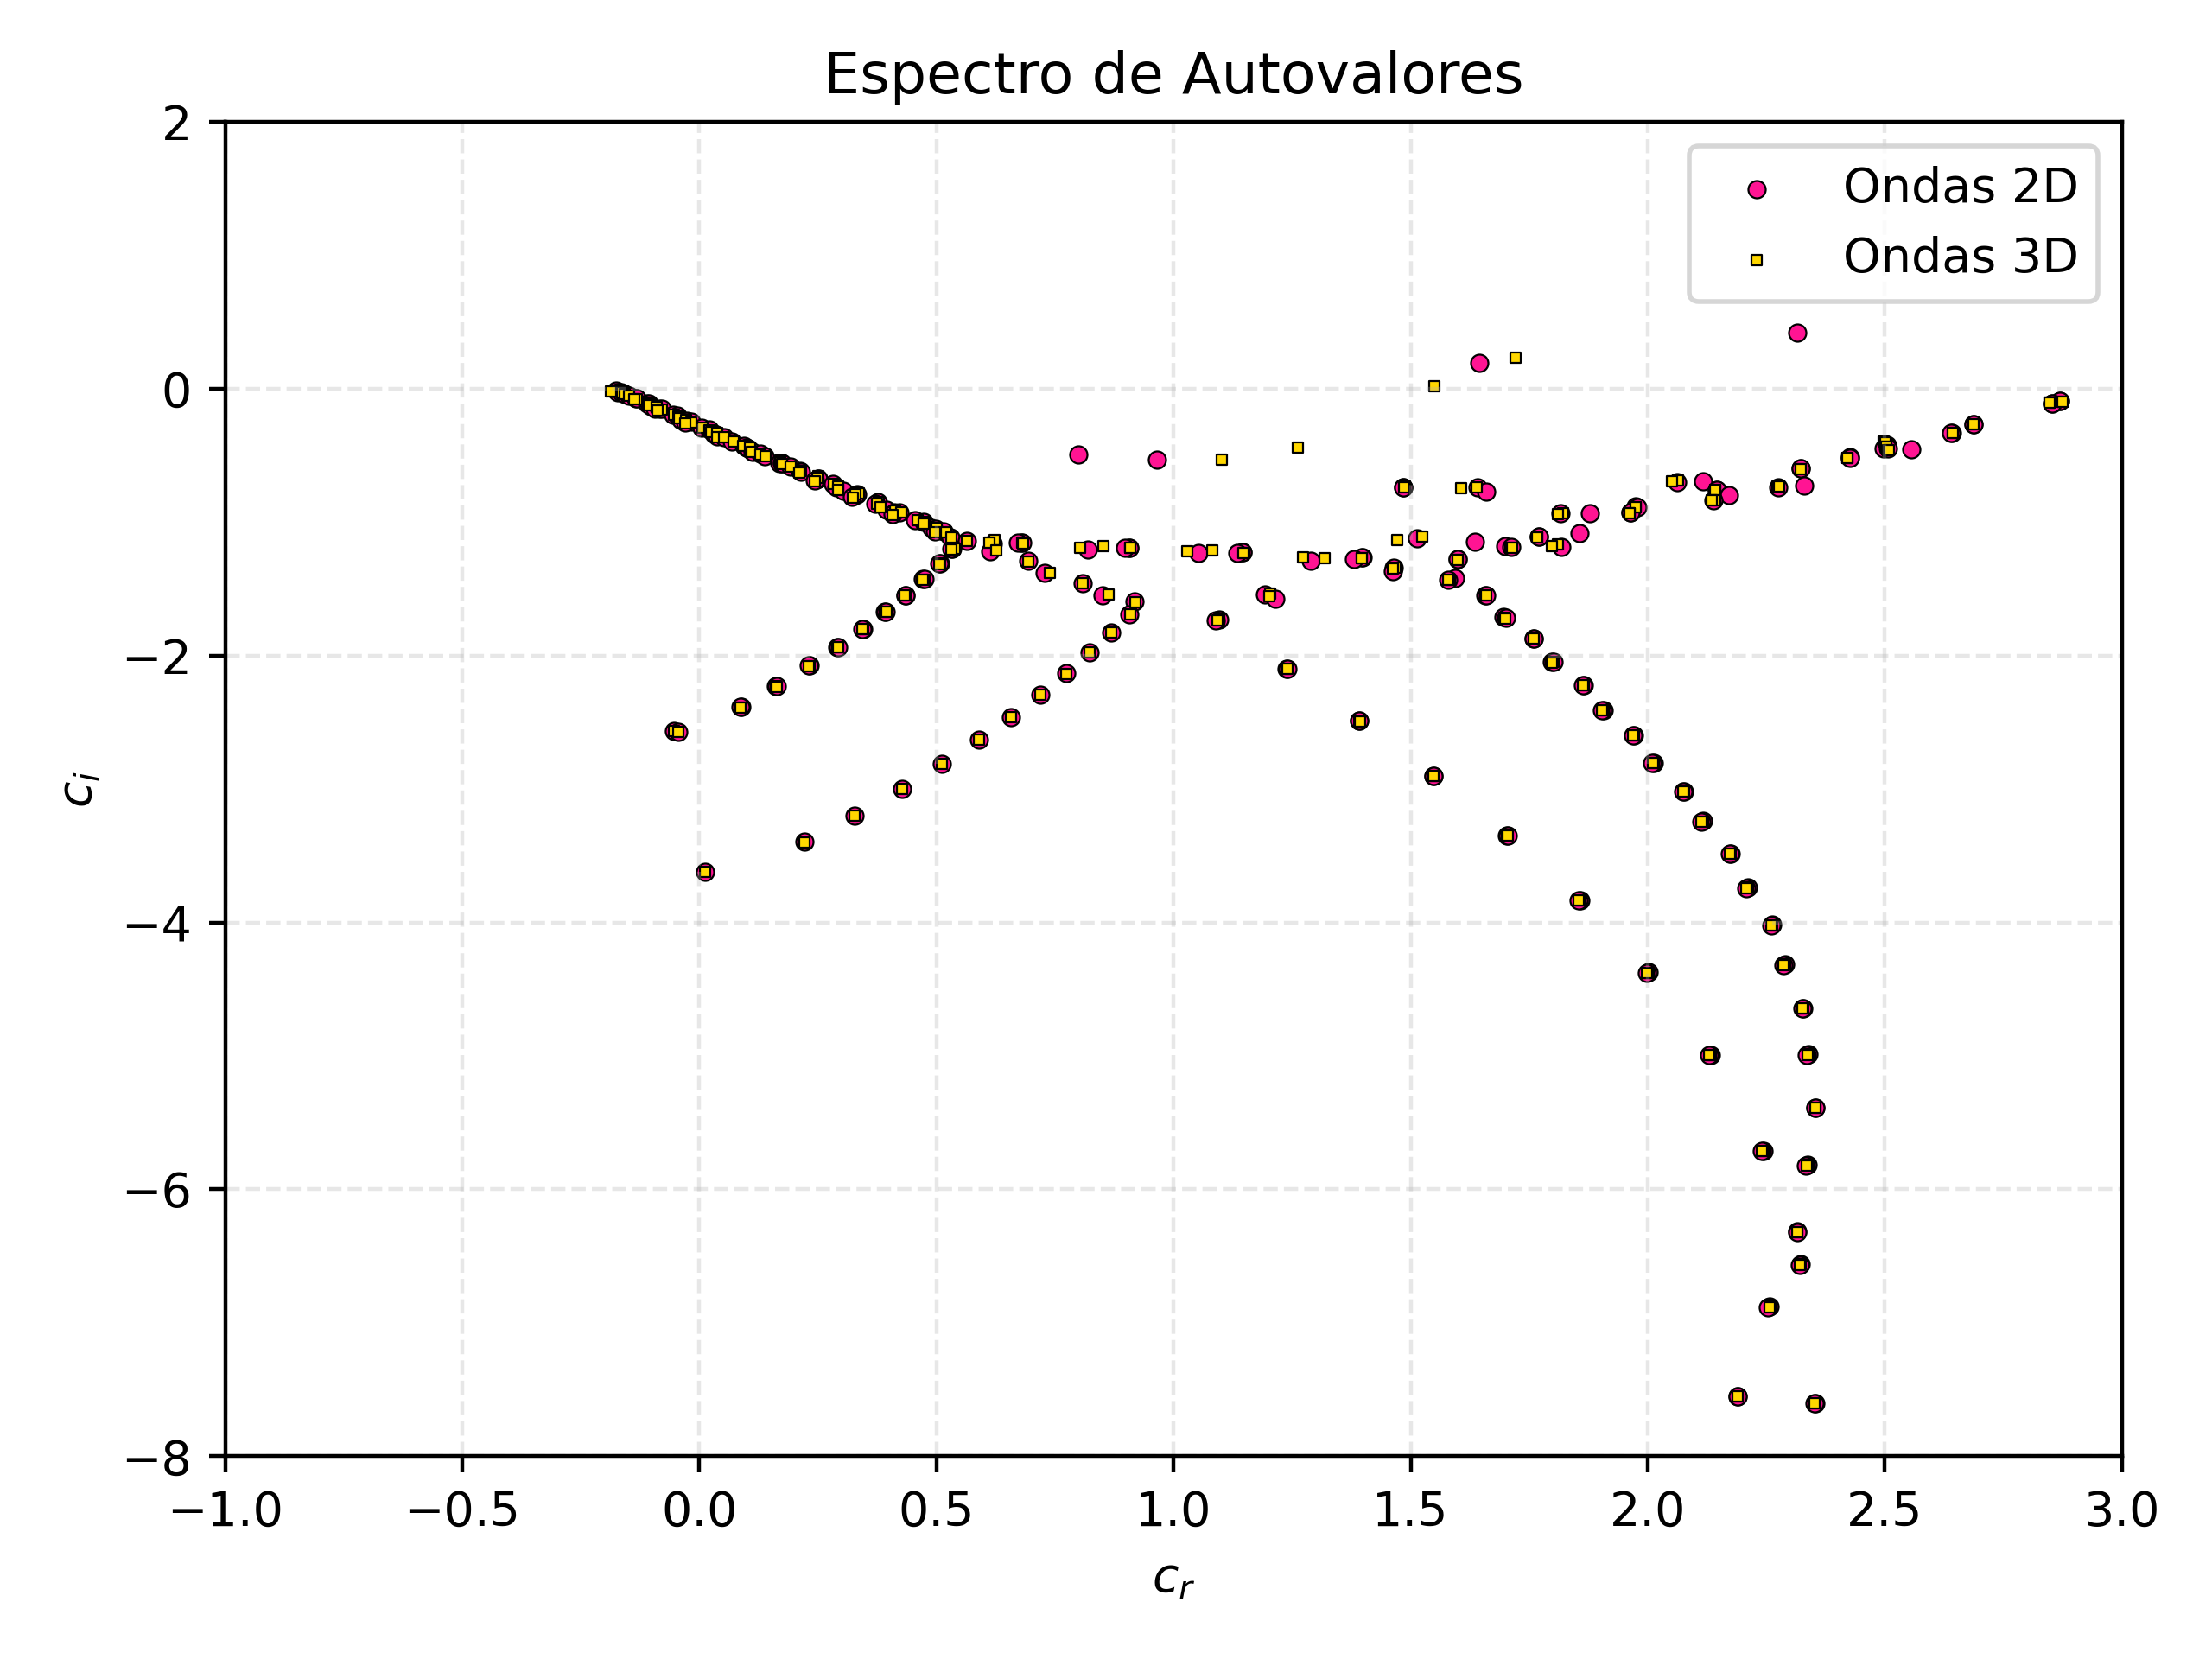
\includegraphics[width=0.6\textwidth]{figures/cap6/Re5000-Pr071-Ri1Em4/Re5000-Pr071-Ri1Em4_eigenvals.png}
  \caption{}
  \label{fig:spectra-Re5000-Pr0071}
\end{figure}


\begin{comment}
\newpage

\section{Casos $\text{Re}=5000$ ; $\text{Pr}=0.71$ ; $\Pi=10^{-3}$}

% =====================
% Tabla 5 – Grupo 5
% =====================
\begin{table}[H]
\centering
\resizebox{\textwidth}{!}{%
\begin{tabular}{lrrrrrrrrr}
\toprule
          Nomenclatura &   Re &   Pr &     Ri &   $\alpha$ & $\beta$ &     A$_{2D}$ &  A$_{3D}$ &             $\lambda_{2D}$ & $\lambda_{3D}$ \\
\midrule
Re5000-Pr071-Ri1Em3-C1 & 5000 & 0.71 & 1E-3 & 1.12 & 0 & 2 $\%$    & 0 $\%$ & 4.376 + 0.704 j & -  \\
Re5000-Pr071-Ri1Em3-C2 & 5000 & 0.71 & 1E-3 & 1.12 & 0 & 1 $\%$    & 0 $\%$ & 4.376 + 0.704 j & -  \\
Re5000-Pr071-Ri1Em3-C3 & 5000 & 0.71 & 1E-3 & 1.12 & 0 & 0.5 $\%$  & 0 $\%$ & 4.376 + 0.704 j & -  \\
Re5000-Pr071-Ri1Em3-C4 & 5000 & 0.71 & 1E-3 & 1.12 & 0 & 0.25 $\%$ & 0 $\%$ & 4.376 + 0.704 j & -  \\
\bottomrule
\end{tabular}}
\caption{}
\label{tab:grupo5}
\end{table}


\subsection{Autofunciones y Espectros de autovalores}

\begin{figure}[H]
  \centering
  \subfloat[]{
    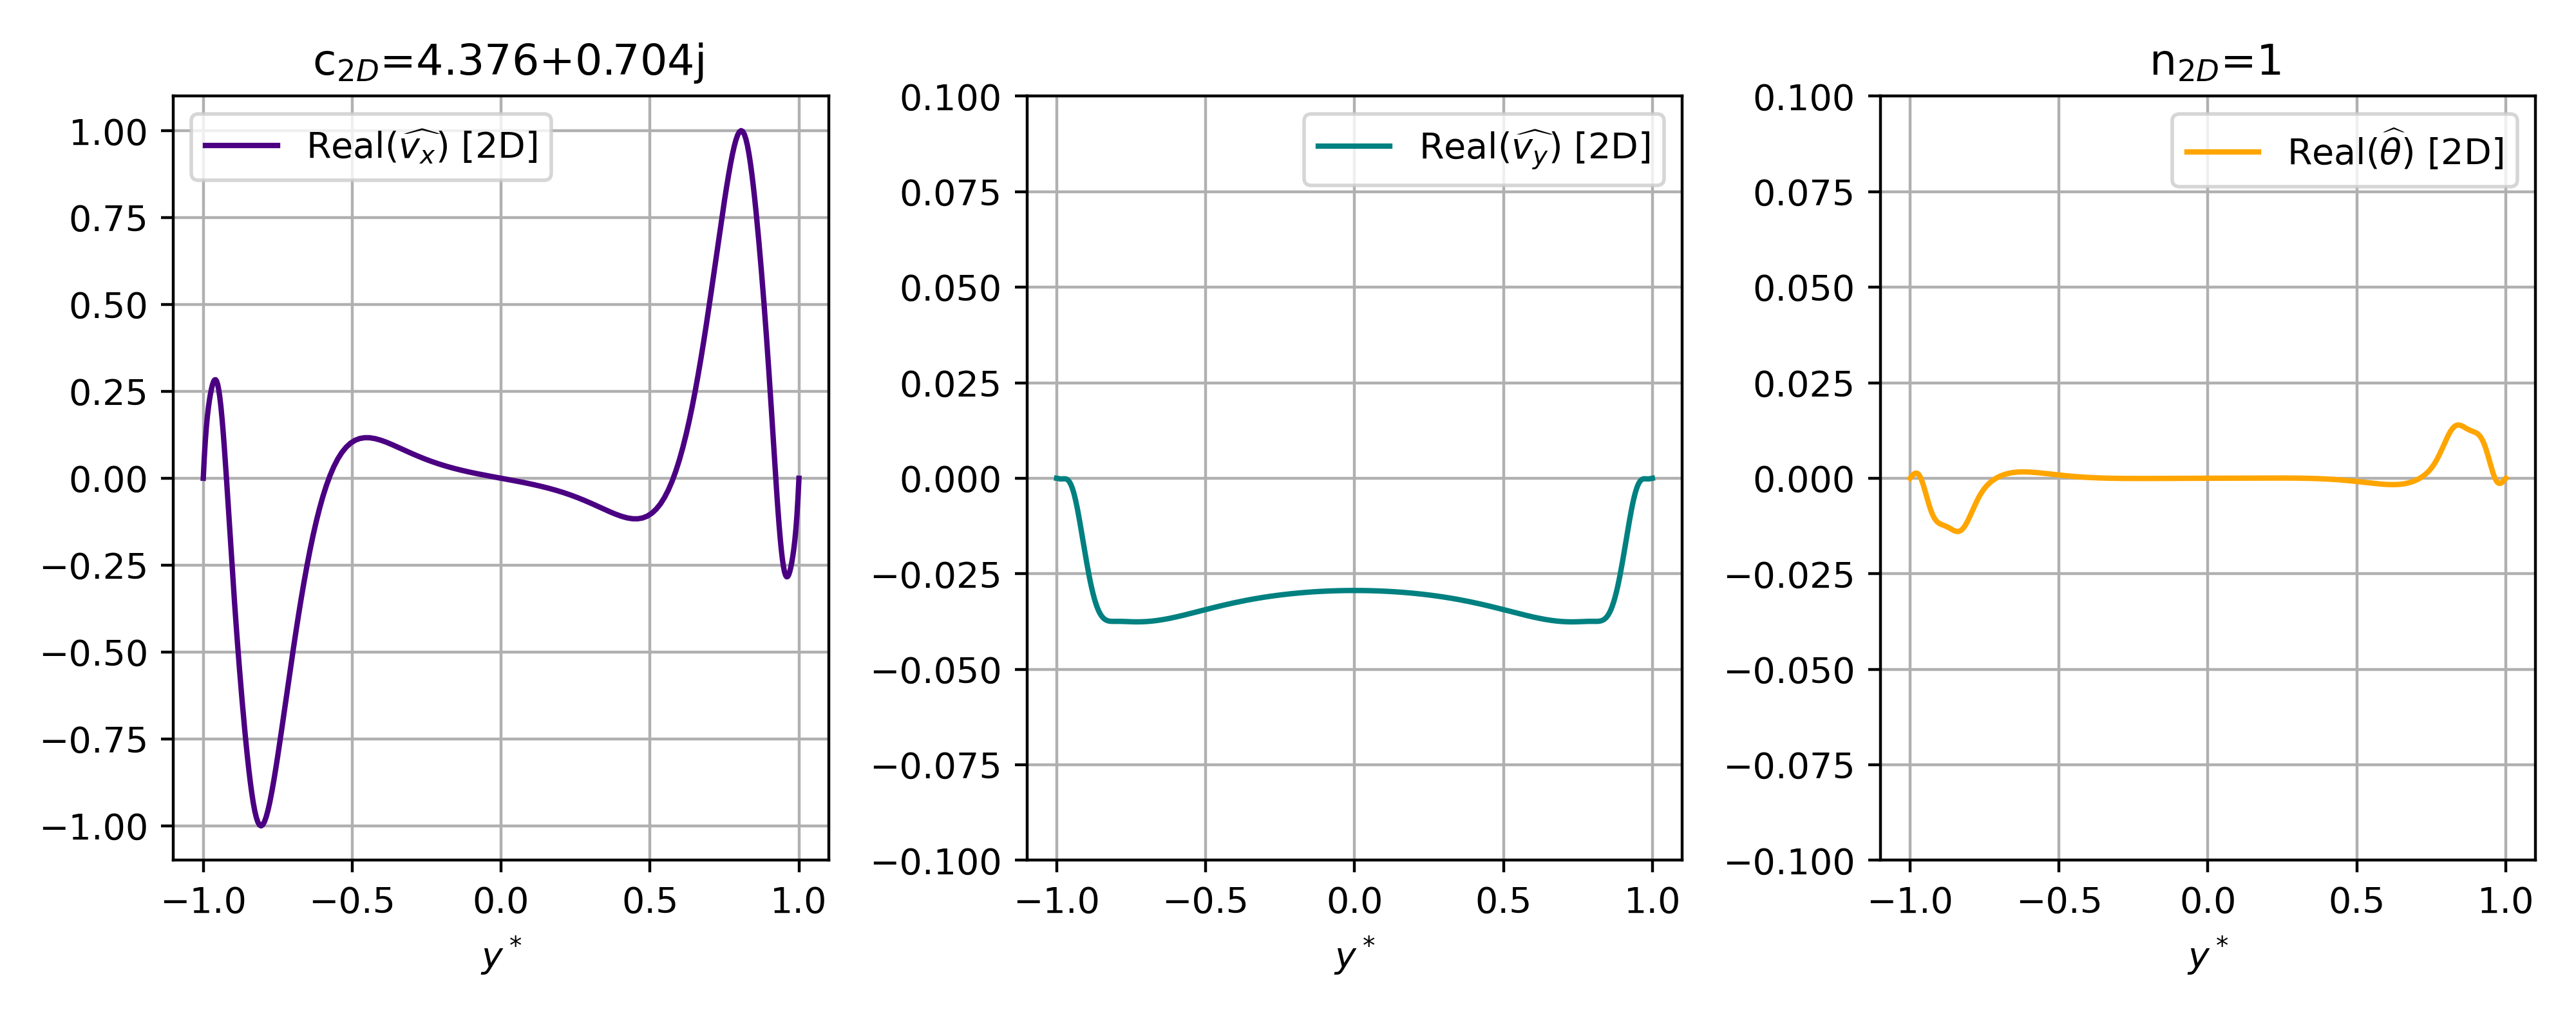
\includegraphics[width=\textwidth]{figures/cap6/Re5000-Pr071-Ri1Em3/Re5000-Pr071-Ri1Em3_eigenfun_A1.png}}
  \caption{}
  \label{fig:eigenfuns1-Re5000-Pr0071}
\end{figure}


\begin{figure}[H]
  \centering
    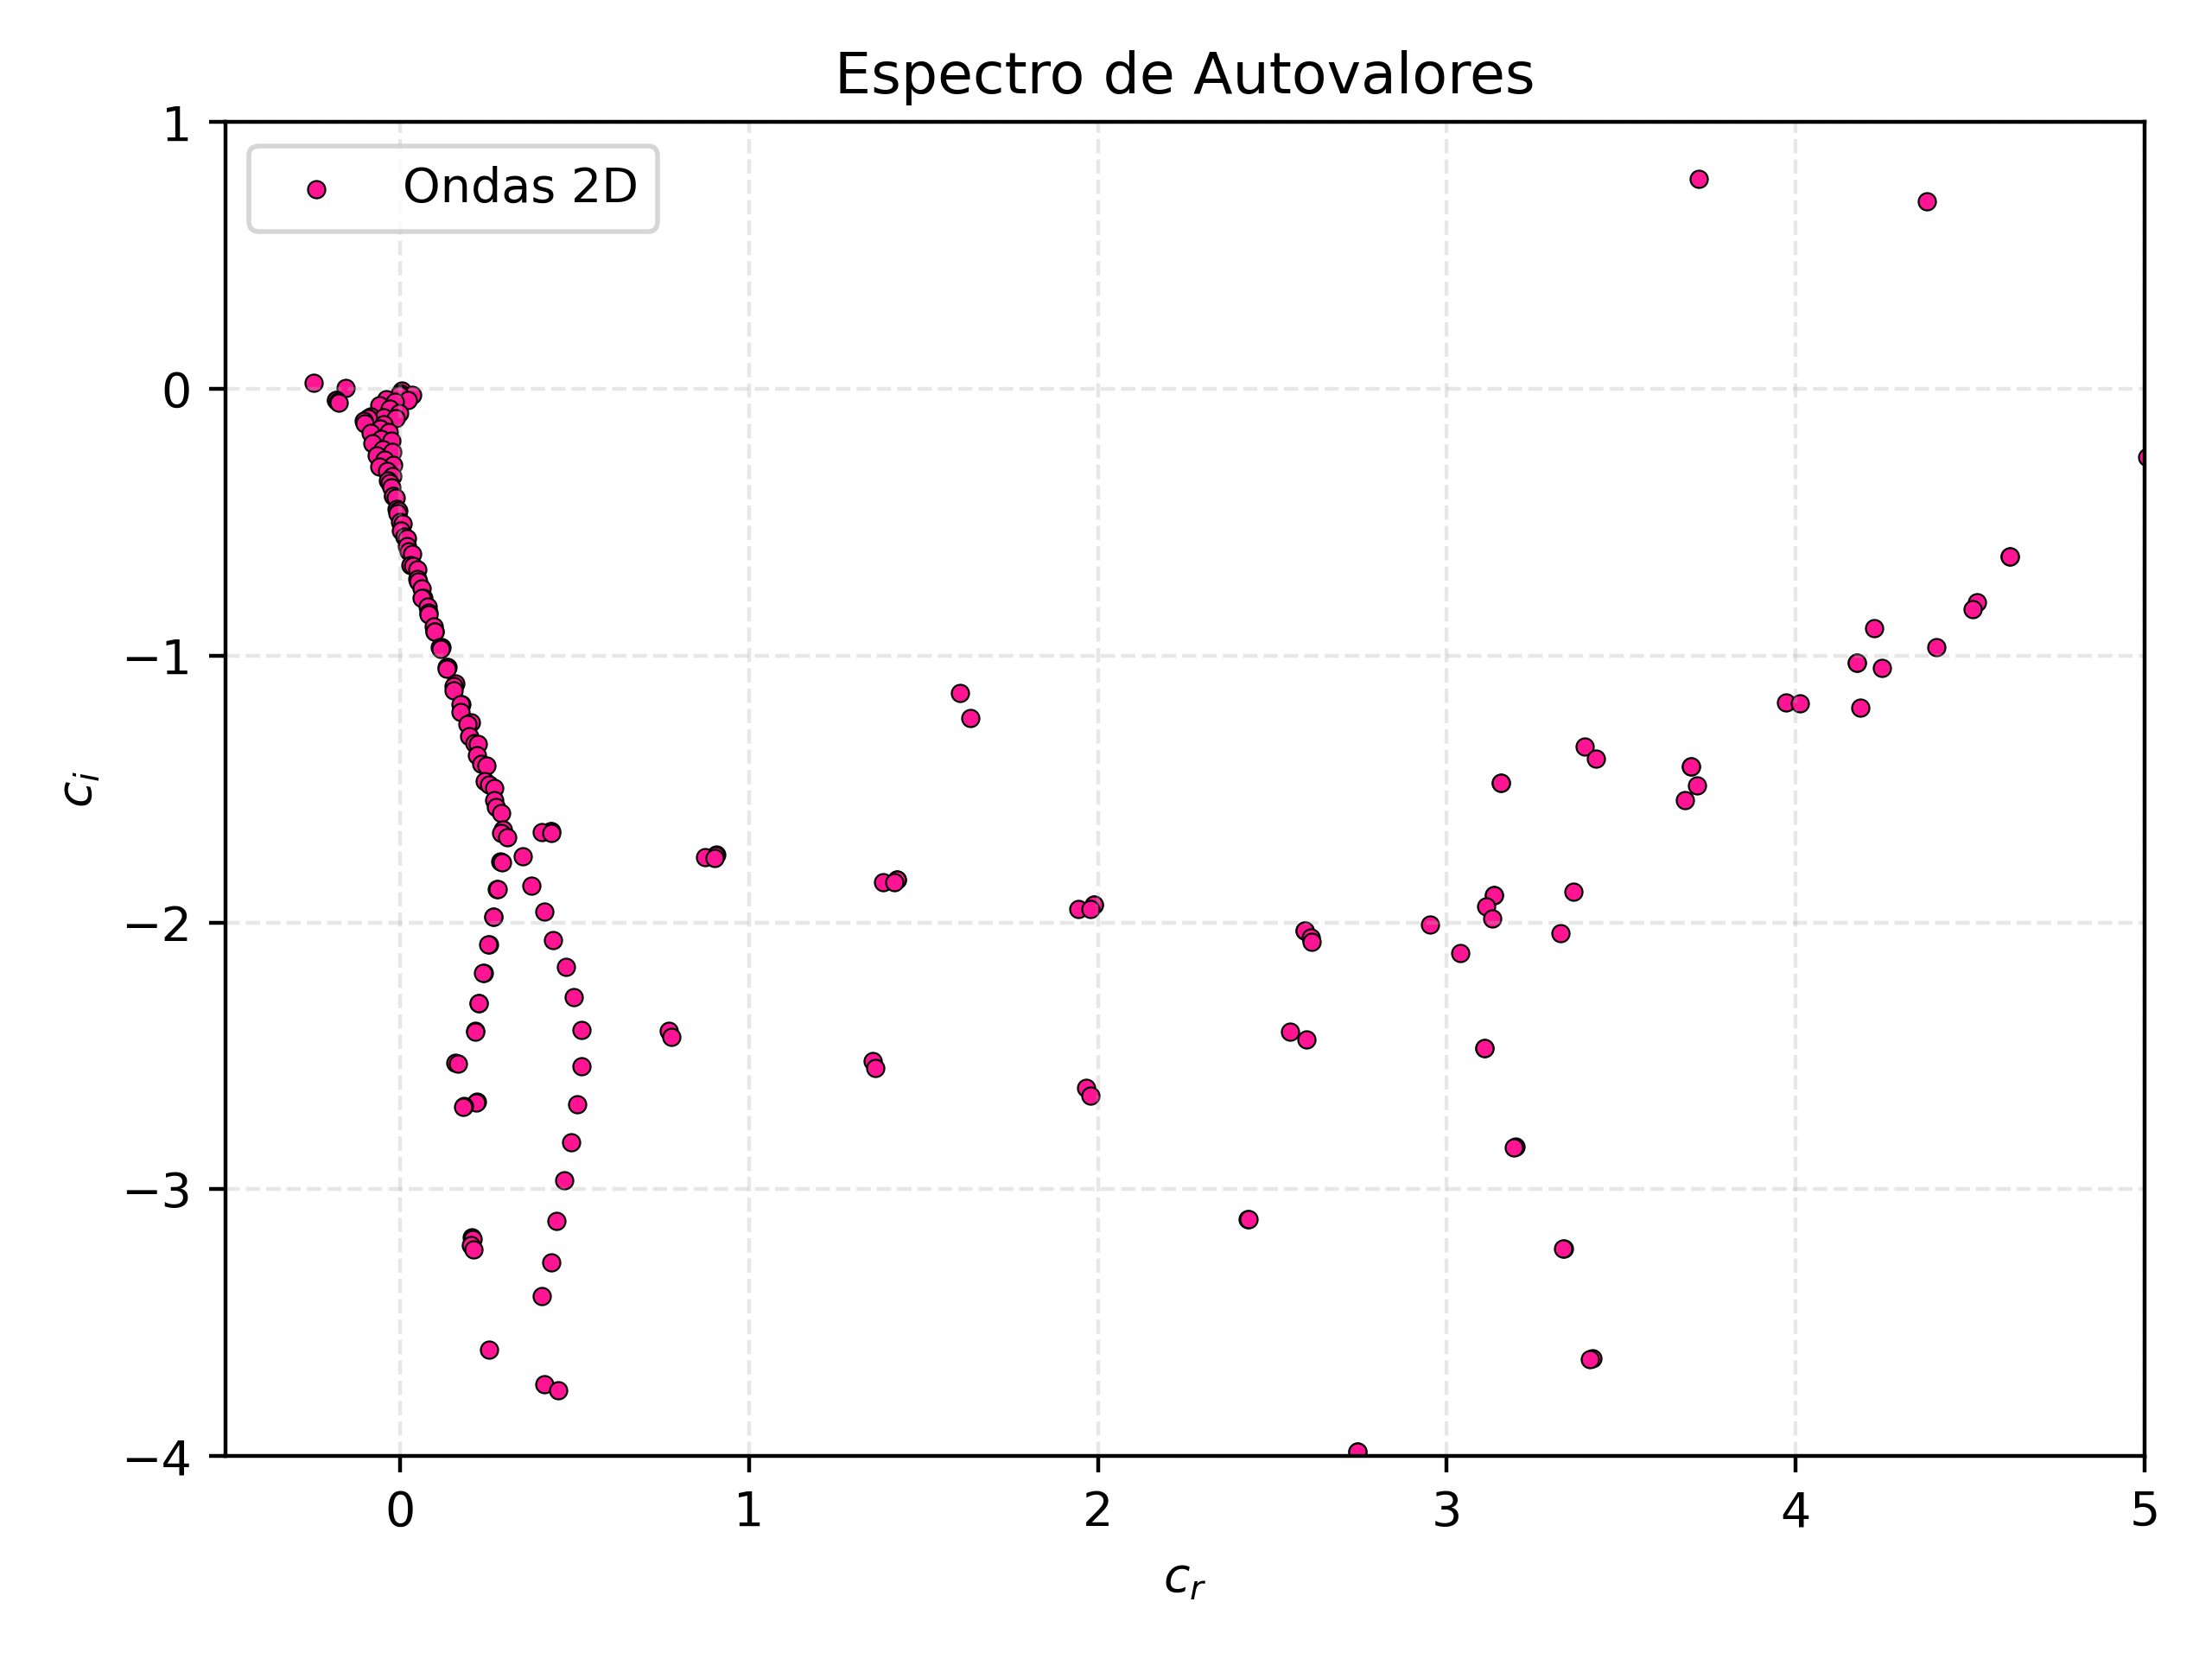
\includegraphics[width=0.6\textwidth]{figures/cap6/Re5000-Pr071-Ri1Em3/Re5000-Pr071-Ri1Em3_eigenvals.png}
  \caption{}
  \label{fig:spectra-Re5000-Pr0071}
\end{figure}


\subsection{TKE, $\langle \theta' \theta' \rangle$, Re$_{\tau}$, Nusselt }

\begin{figure}[H]
  \centering  
  \subfloat[]{
    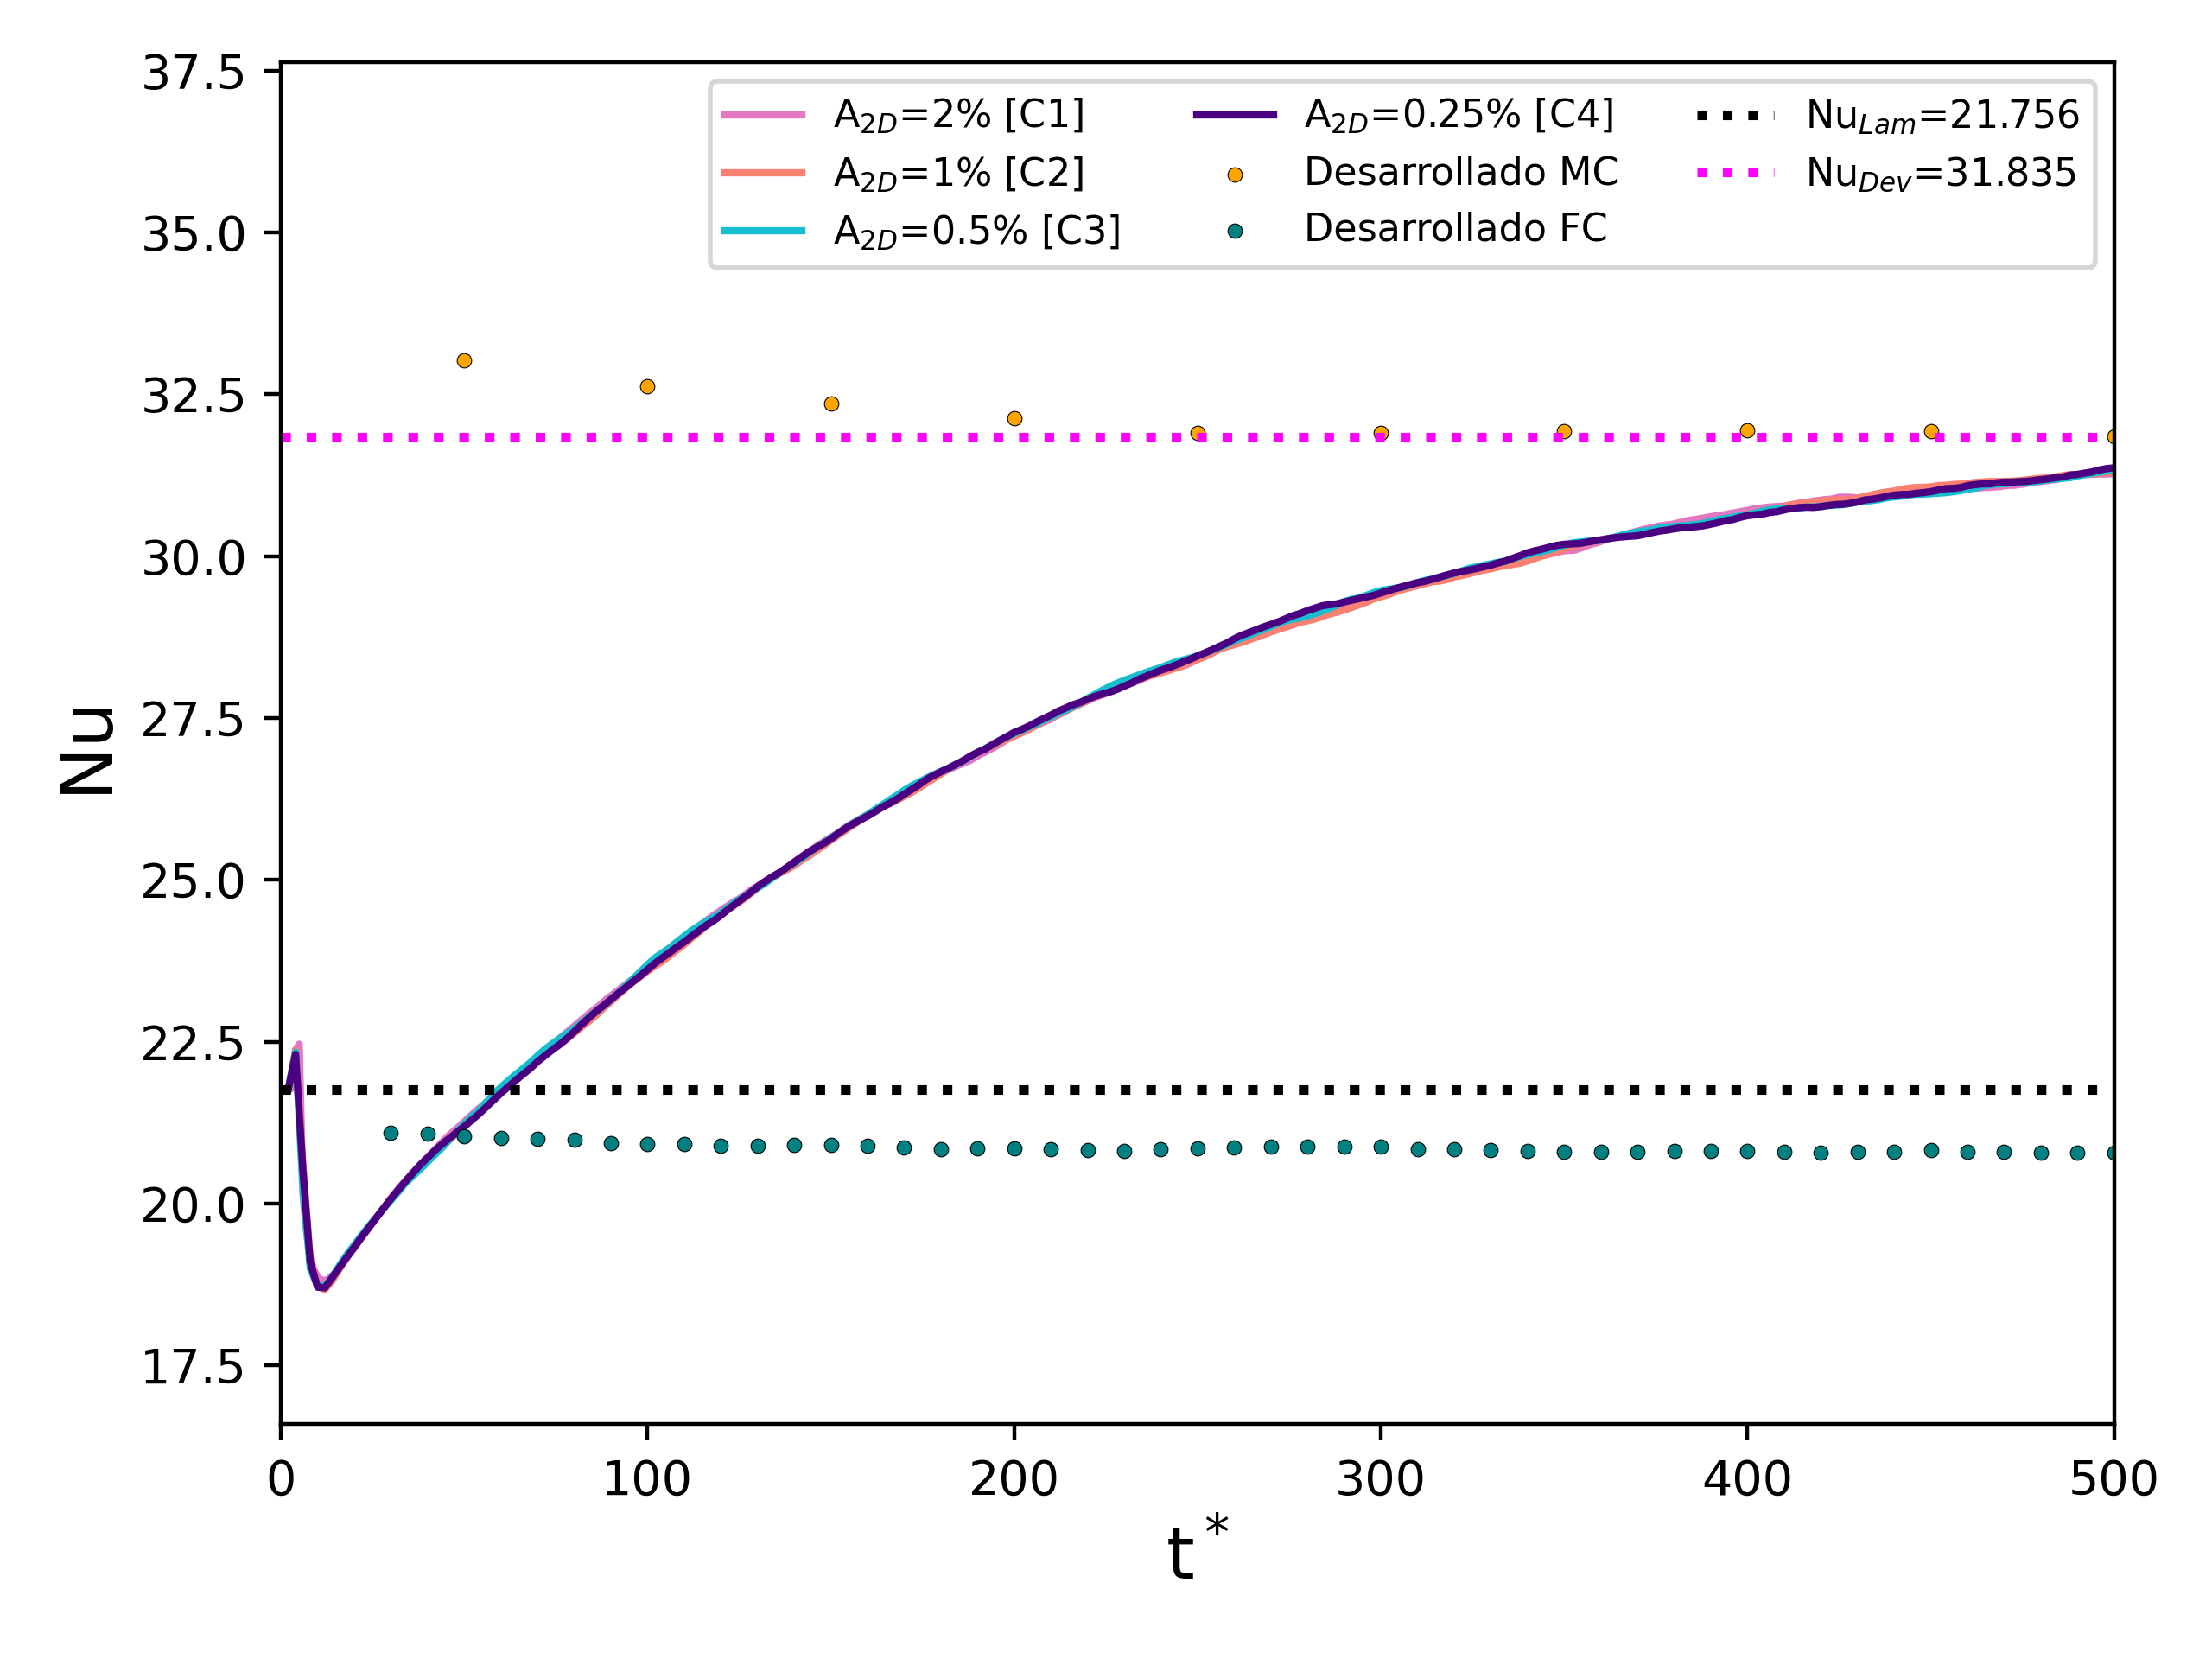
\includegraphics[width=0.49\textwidth]{figures/cap6/Re5000-Pr071-Ri1Em3/Cases_Comp_nussel.png}}
  \subfloat[]{
    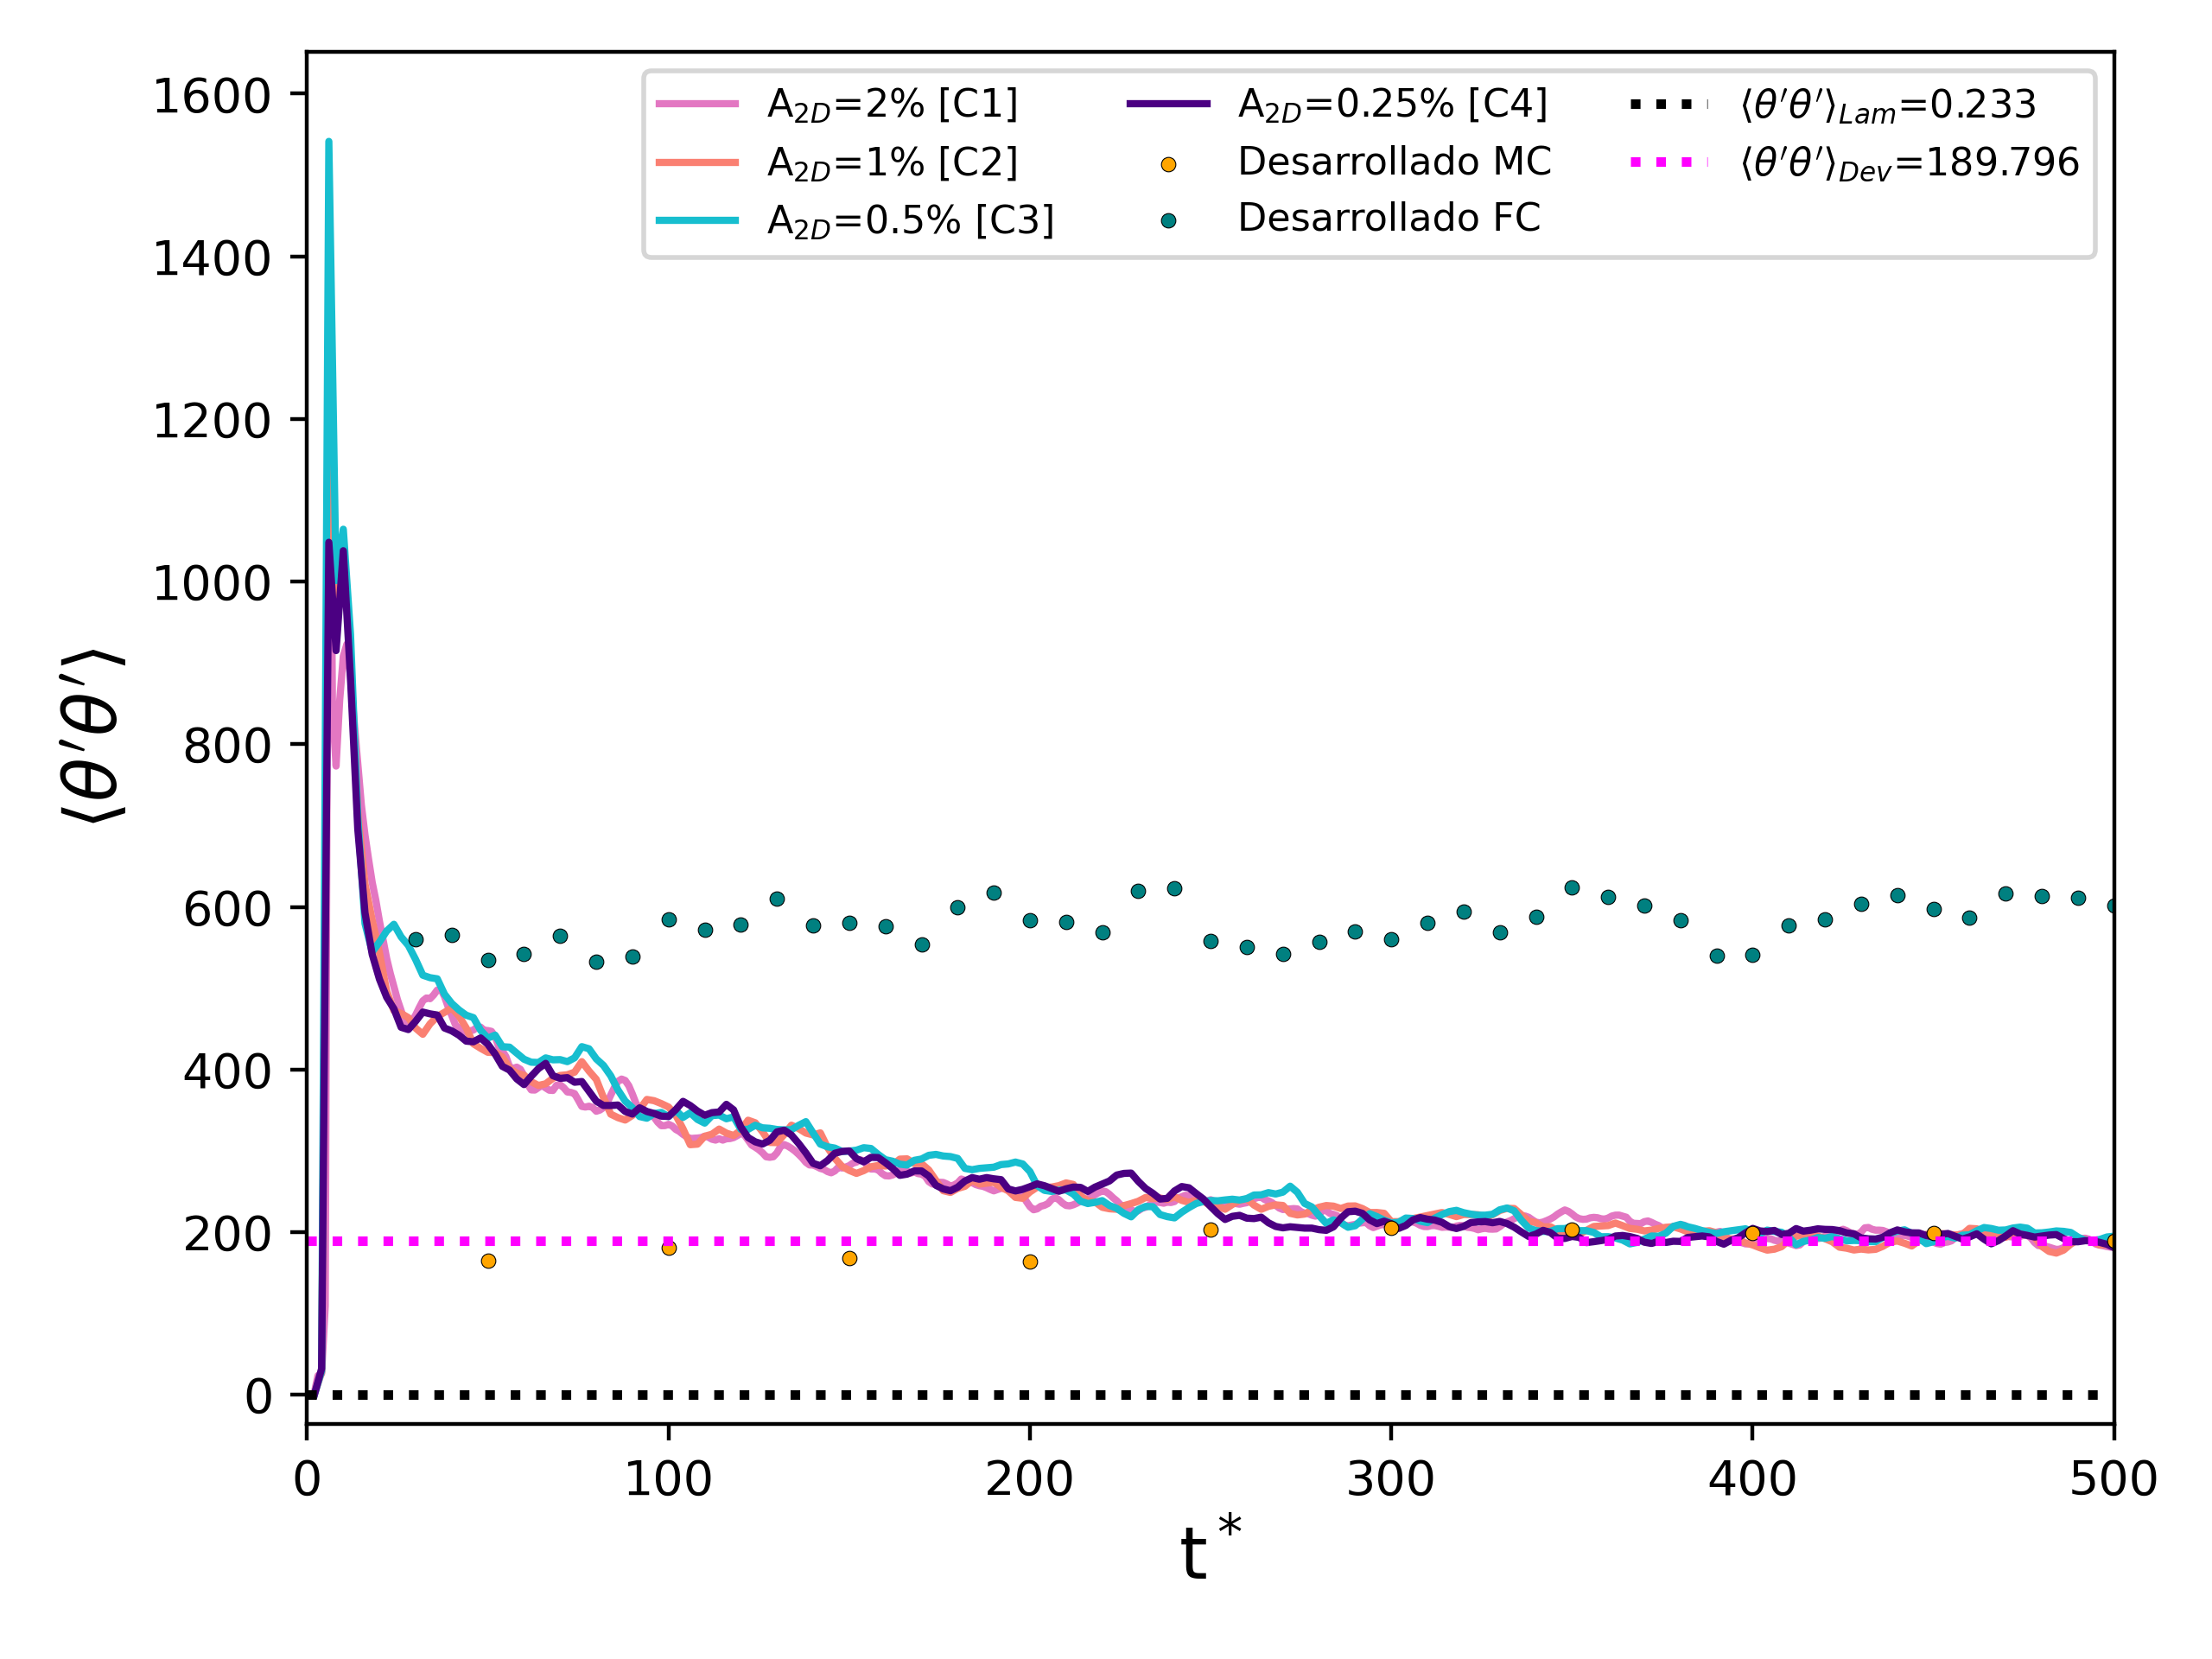
\includegraphics[width=0.49\textwidth]{figures/cap6/Re5000-Pr071-Ri1Em3/Cases_Comp_tetavar.png}}

  \caption{}
  \label{fig:tetavar-nu-Re5000-Pr071-Ri1Em3}
\end{figure}


\begin{figure}[H]
  \centering  
  \subfloat[]{
    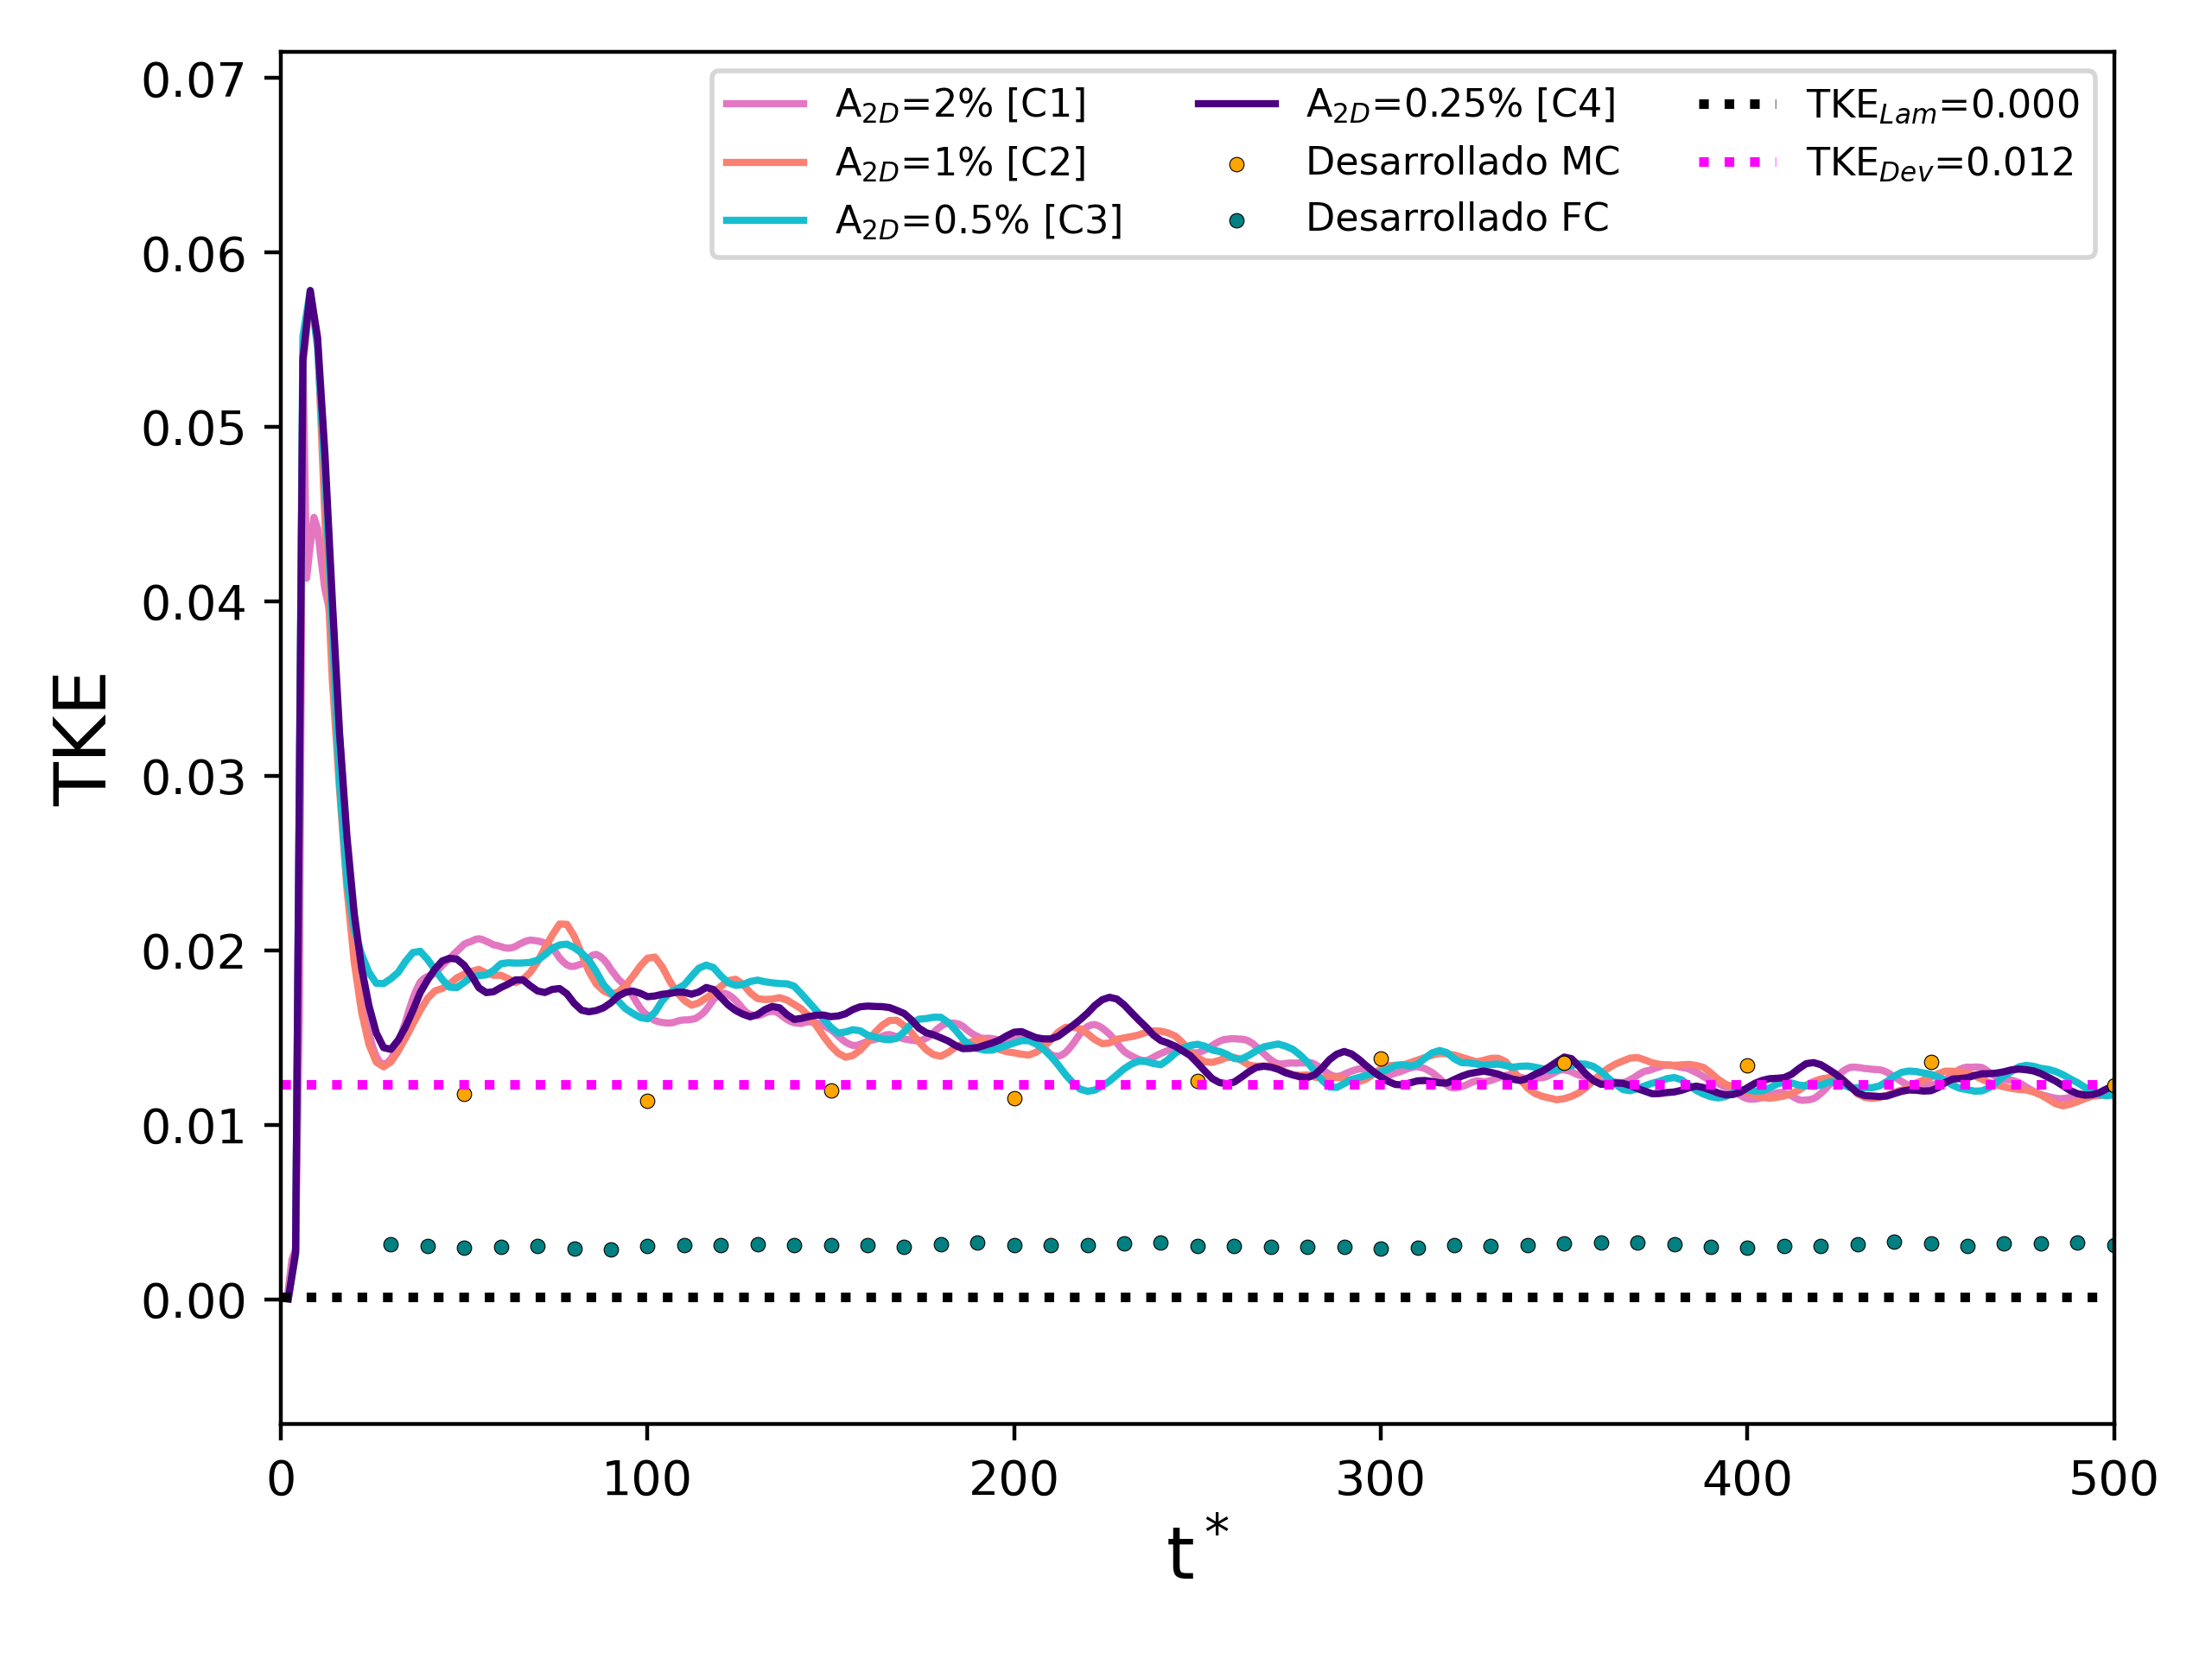
\includegraphics[width=0.49\textwidth]{figures/cap6/Re5000-Pr071-Ri1Em3/Cases_Comp_tke.png}}
  \subfloat[]{
    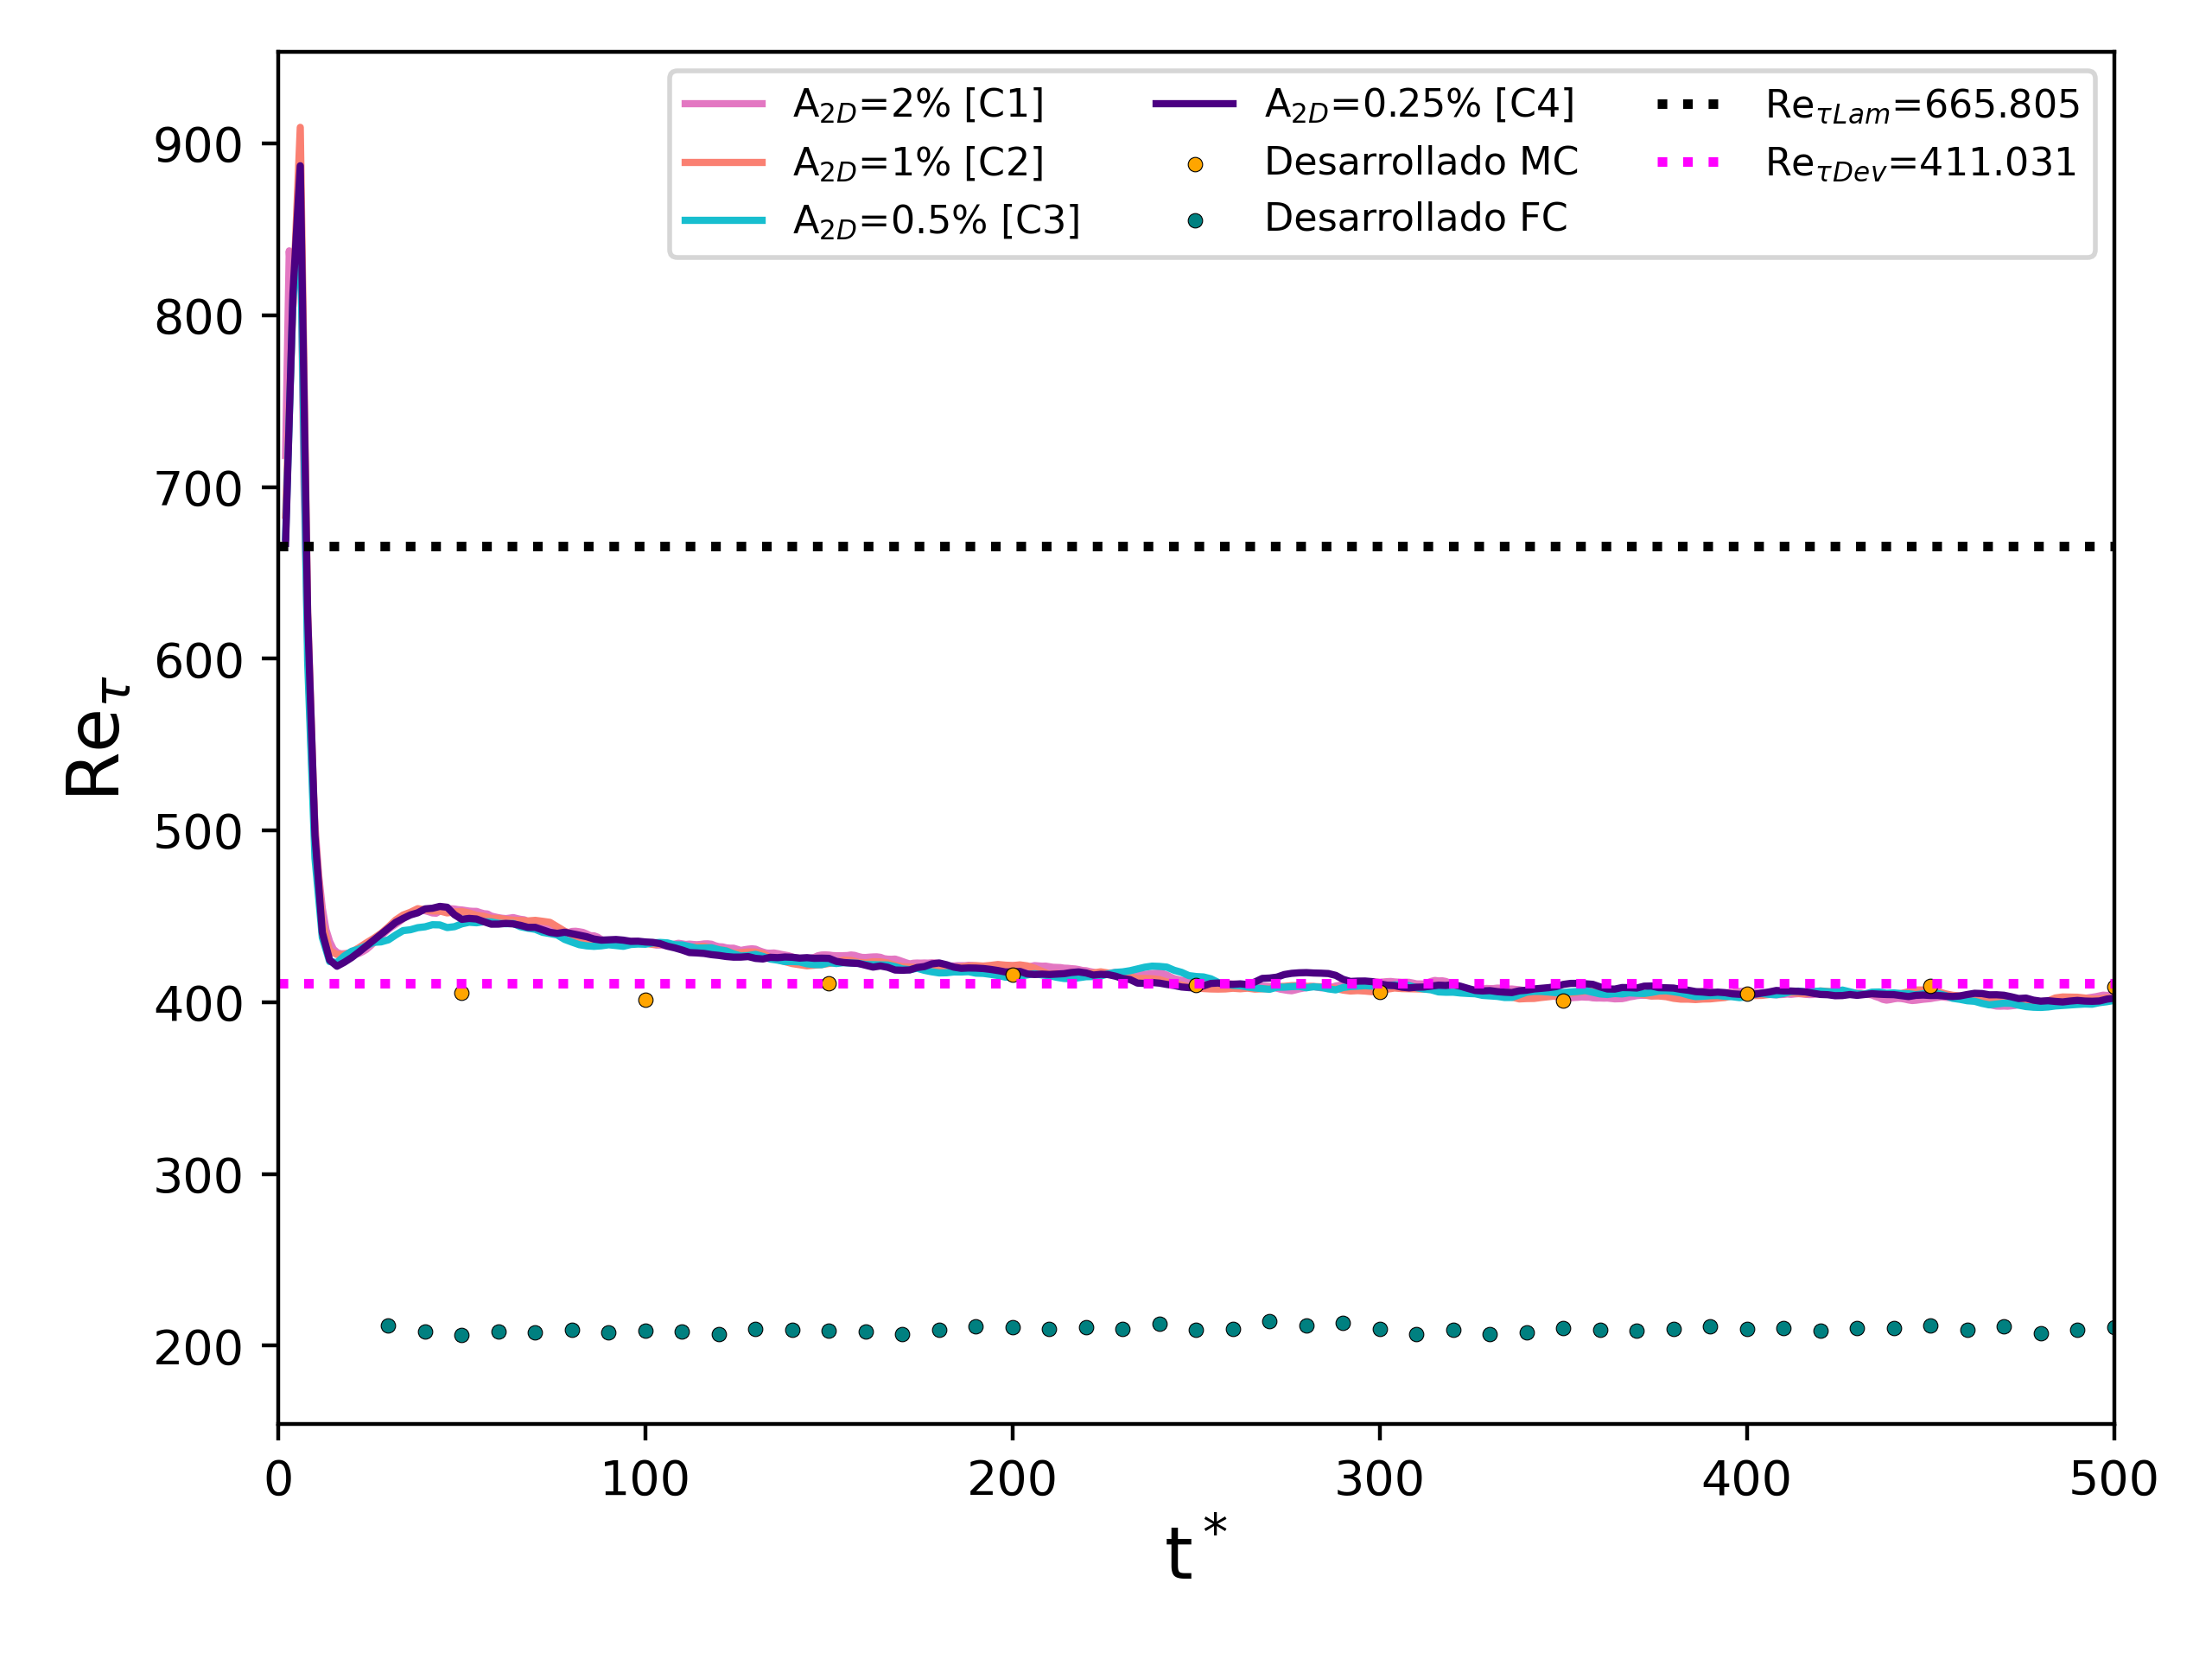
\includegraphics[width=0.49\textwidth]{figures/cap6/Re5000-Pr071-Ri1Em3/Cases_Comp_retau.png}}

  \caption{}
  \label{fig:tke-retau-Re5000-Pr071-Ri1Em3}
\end{figure}
\end{comment}